%%%%%%%%%%%%%%%%%%%%%%%%%%%%%%%%%%%%%%%%%%%%%%%%%%%%%%%%%%%%%%%%%%%%%%%%%%%%
% AGUJournalTemplate.tex: this template file is for articles formatted with LaTeX
%
% This file includes commands and instructions
% given in the order necessary to produce a final output that will
% satisfy AGU requirements, including customized APA reference formatting.
%
% You may copy this file and give it your
% article name, and enter your text.
%
%
% Step 1: Set the \documentclass
%
%

%% To submit your paper:
\documentclass[draft]{agujournal2019}
\usepackage{url} %this package should fix any errors with URLs in refs.
\usepackage{lineno}
\usepackage[inline]{trackchanges} %for better track changes. finalnew option will compile document with changes incorporated.
\usepackage{soul}
\usepackage{amsmath, amssymb}
\usepackage{siunitx}
\usepackage{color}
\usepackage{soul}

\linenumbers
%%%%%%%
% As of 2018 we recommend use of the TrackChanges package to mark revisions.
% The trackchanges package adds five new LaTeX commands:
%
%  \note[editor]{The note}
%  \annote[editor]{Text to annotate}{The note}
%  \add[editor]{Text to add}
%  \remove[editor]{Text to remove}
%  \change[editor]{Text to remove}{Text to add}
%
% complete documentation is here: http://trackchanges.sourceforge.net/
%%%%%%%

\draftfalse

%% Enter journal name below.
%% Choose from this list of Journals:
%
% JGR: Atmospheres
% JGR: Biogeosciences
% JGR: Earth Surface
% JGR: Oceans
% JGR: Planets
% JGR: Solid Earth
% JGR: Space Physics
% Global Biogeochemical Cycles
% Geophysical Research Letters
% Paleoceanography and Paleoclimatology
% Radio Science
% Reviews of Geophysics
% Tectonics
% Space Weather
% Water Resources Research
% Geochemistry, Geophysics, Geosystems
% Journal of Advances in Modeling Earth Systems (JAMES)
% Earth's Future
% Earth and Space Science
% Geohealth
%
% ie, \journalname{Water Resources Research}

\journalname{JGR: Oceans}


\begin{document}

%% ------------------------------------------------------------------------ %%
%  Title
%
% (A title should be specific, informative, and brief. Use
% abbreviations only if they are defined in the abstract. Titles that
% start with general keywords then specific terms are optimized in
% searches)
%
%% ------------------------------------------------------------------------ %%



\title{The Influence of Pine Island Ice Shelf Calving on Melting}

%% ------------------------------------------------------------------------ %%
%
%  AUTHORS AND AFFILIATIONS
%
%% ------------------------------------------------------------------------ %%

% Authors are individuals who have significantly contributed to the
% research and preparation of the article. Group authors are allowed, if
% each author in the group is separately identified in an appendix.)

% List authors by first name or initial followed by last name and
% separated by commas. Use \affil{} to number affiliations, and
% \thanks{} for author notes.
% Additional author notes should be indicated with \thanks{} (for
% example, for current addresses).

% Example: \authors{A. B. Author\affil{1}\thanks{Current address, Antartica}, B. C. Author\affil{2,3}, and D. E.
% Author\affil{3,4}\thanks{Also funded by Monsanto.}}

\authors{A. T. Bradley\affil{1}, D. T. Bett\affil{1}, P. Dutrieux\affil{1}, J. De Rydt\affil{2}, P. R. Holland\affil{1}}


% \affiliation{1}{First Affiliation}
% \affiliation{2}{Second Affiliation}
% \affiliation{3}{Third Affiliation}
% \affiliation{4}{Fourth Affiliation}

\affiliation{1}{British Antarctic Survey, High Cross, Madingley Road, Cambridge CB3 0ET, UK}
\affiliation{2}{Department of Geography and Environmental Sciences, Northumbria University, Newcastle upon Tyne, UK.}

%(repeat as many times as is necessary)

%% Corresponding Author:
% Corresponding author mailing address and e-mail address:

% (include name and email addresses of the corresponding author.  More
% than one corresponding author is allowed in this LaTeX file and for
% publication; but only one corresponding author is allowed in our
% editorial system.)

% Example: \correspondingauthor{First and Last Name}{email@address.edu}

\correspondingauthor{Alexander T. Bradley}{aleey@bas.ac.uk}

%% Keypoints, final entry on title page.

%  List up to three key points (at least one is required)
%  Key Points summarize the main points and conclusions of the article
%  Each must be 100 characters or less with no special characters or punctuation and must be complete sentences

% Example:
\begin{keypoints}
\item	Melting of Pine Island Ice Shelf is sensitive to calving because of a seabed ridge beneath it. 
\item	The melt response to calving has a strong sensitivity on the cavity geometry.
\item	Calving may be an important contribution to the ice-ocean sensitivity of the Antarctic Ice Sheet.
\end{keypoints}

%\begin{keypoints}
%\item
%\item
%\item
%\end{keypoints}

%% ------------------------------------------------------------------------ %%
%
%  ABSTRACT and PLAIN LANGUAGE SUMMARY
%
% A good Abstract will begin with a short description of the problem
% being addressed, briefly describe the new data or analyses, then
% briefly states the main conclusion(s) and how they are supported and
% uncertainties.

% The Plain Language Summary should be written for a broad audience,
% including journalists and the science-interested public, that will not have
% a background in your field.
%
% A Plain Language Summary is required in GRL, JGR: Planets, JGR: Biogeosciences,
% JGR: Oceans, G-Cubed, Reviews of Geophysics, and JAMES.
% see http://sharingscience.agu.org/creating-plain-language-summary/)
%
%% ------------------------------------------------------------------------ %%
\newcommand{\mpryr}{~m~yr\textsuperscript{-1}}


%% \begin{abstract} starts the second page

%\begin{abstract} Observations beneath Pine Island Ice Shelf (PIIS) have revealed the presence of a seabed ridge, which rises several hundred metres above the surrounding bathymetry in places. It is understood that this ridge, in combination with the ice draft above it, form a topographic barrier, restricting access of warm Circumpolar Deep Water to a cavity inshore of the ridge, and thus exerting an important control on basal ablation of the PIIS. In addition, PIIS has experienced several large calving events in recent years, and further calving could significantly alter the cavity geometry. Changes in the ice front location, in combination with changes in ice thickness, might lead to a relaxation of the topographic barrier, and thus significantly change basal melt rates. Here, we consider the impact of past, and possible future, calving events on melt rates of PIIS. We use a high-resolution ocean model to simulate melt rates in both an idealized domain whose geometry captures the salient characteristic features of PIG, and a realistic geometry which accurately resembles it, to explore how changing the ice front position (i.e. calving) affects melt rates. The idealized simulations reveal that the melt response to calving has a sensitive dependence on the thickness of the gap between the ice shelf base and the seabed ridge, with melt rates varying significantly with calving in configurations featuring a narrow ($< 150 $~m) gap, but only weakly for those that feature a wider ($\geq150$~m) gap. The idealized simulations inform our interpretation of the realistic simulations, which demonstrate that modelled melt rates under PIIS do not respond significantly to recent calving events. However, the mean melt rate increases approximately linearly with further calving, with melt rates in the vicinity of the deep grounding line having been amplified by approximately 10\% relative to present day the ice front reaches the ridge crest, a process that will take less than one decade if ice front retreat maintains its present rate. This provides strong evidence that the impact of calving may represent an important, but as yet unexplored, contribution to the ice-ocean sensitivity of the West Antarctic Ice Sheet.
%\end{abstract}

\begin{abstract}
    A seabed ridge beneath Pine Island Ice Shelf (PIIS), in combination with the ice draft above it, form a topographic barrier, restricting access of warm Circumpolar Deep Water to a cavity inshore of the ridge, and thus exerting an important control on basal ablation of the PIIS. In addition, PIIS has experienced several large calving events in recent years, and further calving could significantly alter the cavity geometry. Changes in the ice front location, in combination with changes in ice thickness, might lead to a relaxation of the topographic barrier, and thus significantly change basal melt rates. Here, we consider the impact of past, and possible future, calving events on melt rates of PIIS. We use a high-resolution ocean model to simulate melt rates in both an idealized domain whose geometry captures the salient characteristic features of PIG, and a realistic geometry which accurately resembles it, to explore how changing the ice front position (i.e. calving) affects melt rates. The idealized simulations reveal that the melt response to calving has a sensitive dependence on the thickness of the gap between the ice shelf base and the seabed ridge and inform our interpretation of the realistic simulations, which demonstrate that modelled melt rates under PIIS do not respond significantly to recent calving events. However, the mean melt rate increases approximately linearly with further calving, and are amplified by approximately 10\% relative to present day the ice front reaches the ridge crest, which will take less than one decade if ice front retreat maintains its present rate. This provides strong evidence that the impact of calving may represent an important, but as yet unexplored, contribution to the ice-ocean sensitivity of the West Antarctic Ice Sheet.
\end{abstract}

\section*{Plain Language Summary}
Pine Island Glacier has a large seabed ridge beneath its floating extension, referred to as Pine Island Ice Shelf. The combination of the ridge and ice shelf above it reduce the amount of relatively warm water that is able to reach the ice shelf, therefore restricting its melting. However, the ice shelf has also lost large sections from its front in recent years, in a process referred to as calving. In this paper, we investigate the effect of these two processes: how does calving affect the melt rates on Pine Island Ice Shelf. Using numerical simulations of the ocean flow beneath the ice shelf, we identify a potentially high sensitivity of melt rates on calving, depending on the cavity geometry. In addition, our simulations suggest that the melt rate has an approximately linear dependence on the distance that the ice front retreats after any further calving events. These results provide strong evidence that changes in the melting of ice shelves in response to calving might represent an important contribution to the response of West Antarctica in a changing climate.


%% ------------------------------------------------------------------------ %%
%
%  TEXT
%
%% ------------------------------------------------------------------------ %%
\section{Introduction}\label{S:Introduction}
Pine Island Glacier (PIG), located in the Amundsen Sea sector of Antarctica, is one of the fastest changing glaciers worldwide. A sustained increase in ice discharge and surface velocity, as well as significant grounding line retreat, have been documented since satellite measurements began in the 1990s \cite{Rignot2002AnnGlac, Rignot2008GRL, Rignot2011Science, Mouginot2014GRL, Gardner2018Cryo}. PIG has experienced a 70\% increase in grounding line ice flux and a close to doubling of surface velocity between 1974 and 2013 \cite{Mouginot2014GRL}, while its grounding line retreated some 31~km at its centre between 1992 and 2011 \cite{Rignot2014GRL}. Increased basal melting of Pine Island Ice Shelf (PIIS) -- the floating extension of the PIG's grounded ice -- has been implicated as a key driver of these changes \cite{Shepherd2004GRL, Pritchard2012Nature, Rignot2019PNAS}: ice shelves offer a resistive stress (commonly referred to as `buttressing') that restrains the flow of grounded ice; increased basal melting can reduce ice shelf volume and thus the buttressing they are able to provide \cite{Gudmundsson2013Cryo, Reese2018NatureClimCh, Gudmundsson2019GRL,Gagliardini2010GRL,Goldberg2019GRL, DeRydt2021Cryosphere}.

%depth of the pycnocline is the most important factor
In the Amundsen Sea sector, Circumpolar Deep Water (CDW) provides the main source of heat that drives ice shelf melting. The pycnocline that separates CDW from Winter Water above it remains mostly above the level of the continental shelf break in the Amundsen Sea \cite{Jacobs2015Oceanography, Heywood2016Oceanography}. CDW is therefore able to spill onto the continental shelf and reach ice shelf cavities, providing significant heat to the adjacent ice shelves for melting. The flux of CDW that is able to spill over the continental shelf is a good proxy for the depth of this pycnocline; this flux (and thus the depth of the pycnocline) is not constant, but varies significantly on decadal timescales \cite{Jenkins2018NatureGeo}. Years with a deeper pycnocline, and thus thinner CDW layer, tend to result in lower meltwater fluxes from ice shelves, and vice versa~\cite{Jacobs2011NatureGeosci,Dutrieux2014Science}.

\begin{figure}
    \centering
    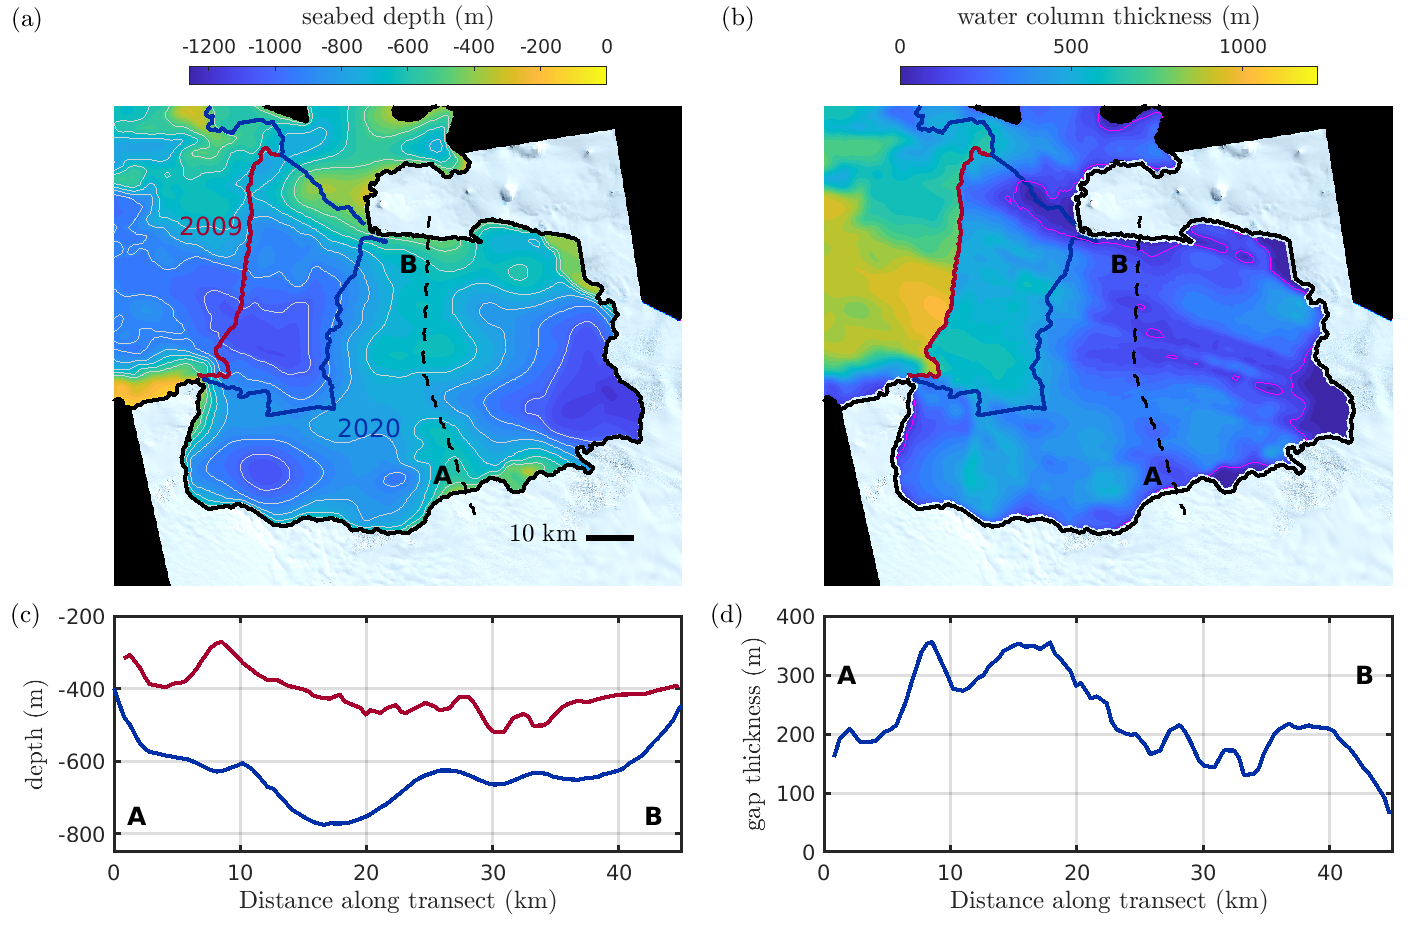
\includegraphics[width = \textwidth]{../make_figures/plots/figure1.png}
    \caption{(a) Seabed depth and (b) water column thickness under Pine Island Ice Shelf and in Pine Island Bay (colors) from~\citeA{Dutrieux2014Science}. Also shown are the locations of the ice front in 2009 (red line) and 2020 (blue line), as indicated in (a).  The solid black line indicates the grounding line from \citeA{Joughin2010GRL}, and the background image is a Sentinel 2 mosaic from November 2020. The black dashed line indicates the approximate location of the crest of the seabed ridge. The magenta contour in (b) corresponds to 125~m  water column thickness. (c) Seabed bathymetry (blue) and ice draft (red) taken along the black dashed line in (a)--(b). (d) Plot of the ridge-draft gap measured along the black dashed black line in (a) [i.e. the difference between the red and blue lines in (c)]. }
    \label{fig:figure1}
\end{figure}


%ridge in PIG makes pycnocline picture more complicated
However, for PIG specifically, this simple `pycnocline depth' picture is complicated by the presence of a seabed ridge in the ice shelf cavity. This ridge is located several tens of kilometers downstream of the grounding line, and protrudes up to three hundred meters above the neighboring seabed (figure~\ref{fig:figure1}a). In combination with the ice shelf directly above it, the ridge acts as a topographic barrier, restricting the access of CDW to an inner cavity which has formed between the ridge and the ice shelf since the grounding line retreated from this ridge in a process initiated in the late 1940s~\cite{Jenkins2010NatureGeo, DeRydt2014JGeophysResOceans, DeRydt2016JGeophysResEarthSurf, Smith2017Nature}. This cavity geometry means that, at present, the strength of the topographic barrier (i.e. how much its presence affects ice shelf melting) is strongly dependent on the pycnocline depth: at its shallowest, the pycnocline sits above the depth of the ridge crest, and a large amount of modified CDW is able to spill into the inner cavity~\cite{Dutrieux2014Science}; in contrast, at its lowest, the pycnocline sits some way below the ridge crest and CDW access is severely restricted.  The presence of the seabed ridge thus contributes to the strong sensitivity of PIIS melting to hydrographic conditions in Pine Island Bay (PIB): \citeA{Dutrieux2014Science} reported that the total freshwater flux from the fast flowing part of PIG in 2009 (80~km\textsuperscript{3}), when the pycnocline was at its shallowest depth on record~\cite{Webber2017NatureComms}, was more than double its value in 2012 (37~km\textsuperscript{3}), when the pycnocline was at the second-lowest recorded depth.

%another thing we have seen is significant calving events
In addition to its unique topographic control on melt rates, the recent calving of PIIS also stands out amongst Amundsen Sea terminating ice shelves. Mass loss from the Antarctic ice sheet is dominated by calving and melting~\cite{Rignot2013Science}; in equilibrium, these losses must balance the upstream accumulation of ice. The recent retreat of the ice front of PIIS, however, suggests that the calving rate is far higher than would be required to maintain an equilibrium. The ice front retreated approximately 26 km between 2009 and 2020 (figure~\ref{fig:figure1}a), with the majority of this retreat happening over the period 2015--2020~\cite{Lhermitte2020PNAS, Joughin2021ScienceAdv} This corresponds to a more-than-doubling of the calving rate, from approximately 4~km~year\textsuperscript{-1} prior to 2015, to approximately 9~km~year\textsuperscript{-1} in the period 2015--2020 [the flow speed at the ice front, for context, is approximately 5~km~year\textsuperscript{-1} \cite{Joughin2021ScienceAdv}].

%at present, the ridge is located approx x km downstream of the ridge crest. The changes some far have been implicated in a speed up because of a loss of buttressing, but might the changes have also led to a relaxation of the topographic barrier and thus and increase in melt rates (that would only be evidenced on longer timescales(?)) [key question one]
As of 2020, the ice front is located approximately 20~km downstream of the ridge (figure~\ref{fig:figure1}a), meaning that the ice front is now closer to the ridge crest than it is to the location of the ice front in 2009. The loss of buttressing associated with this retreat of the ice front can explain the acceleration of PIG since 2015~\cite{Joughin2021ScienceAdv}. However, given that the topographic barrier to CDW relies on the combination of ice draft \textit{and} seabed ridge, the recent calving events beg the following question: has recent calving of PIIS relaxed the topographic barrier, leading to significant changes in melting? Increased melting of its ice shelf might lead to further reductions in ice shelf volume and thus reduced buttressing, ultimately leading to ice shelf acceleration, thinning, and grounding line retreat.

%but also, in future, we might have further calving events because or preconditioning and or MICI that might bring to ridge to the crest. How might these potential future calving events lead to changes in melt rates? [key question two]
In addition to considering the effect on melt rates of calving events that have already happened, one might also consider how melt rates might respond to possible future calving events. It has been suggested that further significant calving of PIIS is likely, since damage to the ice shelf that has already occurred is thought to have preconditioned PIIS to collapse~\cite{Lhermitte2020PNAS}. Furthermore, if calving does indeed affect melting, one could imagine a `calving-melting' feedback loop in which calving enhances ice shelf melting, leading to reduced buttressing and thus ice acceleration, ultimately resulting in ice shelf damage and further calving. Here, we test the first link in this chain of events.

In this study, we assess how, and why, melt rates on PIIS might respond to past, and possible future, calving events. To do so, we use a numerical general circulation model to simulate the ocean circulation in both an idealized setup whose geometry captures the salient characteristic features of PIIS and its cavity (most notably, a seabed ridge whose crest is in proximity to the ice shelf base), and a realistic setup whose geometry closely matches real world conditions for PIIS. We begin in \S\ref{S:Experiment} with a description of the idealized experiments, setting out details of the ocean model used and the experimental setup. We identify one such experiment as a baseline, and present the results of this experiment in \S\ref{S:Baseline}. In \S\ref{S:Results:lc}, we describe how, and why, the melt rate varies as calving proceeds from this baseline. In the following two sections, we discuss how the picture of melt response to calving presented in \S\ref{S:Results:lc} changes when the cavity geometry (\S\ref{S:Results:H}) and far field ocean conditions (\S\ref{S:Results:P}) are altered. In \S\ref{S:Realistic} we describe and present the results of  the realistic experiments. Guided by the results of the idealized experiments, we assess the expected response of melt rates under PIIS to recent, and possible future, calving events. Finally, we discuss the implications of our results in \S\ref{S:Discussion}, and summarize the key results in \S\ref{S:Summary}.


\section{Idealized Experiment Details}\label{S:Experiment}
%broad overview of the experiemnts

\begin{figure}
    \centering
    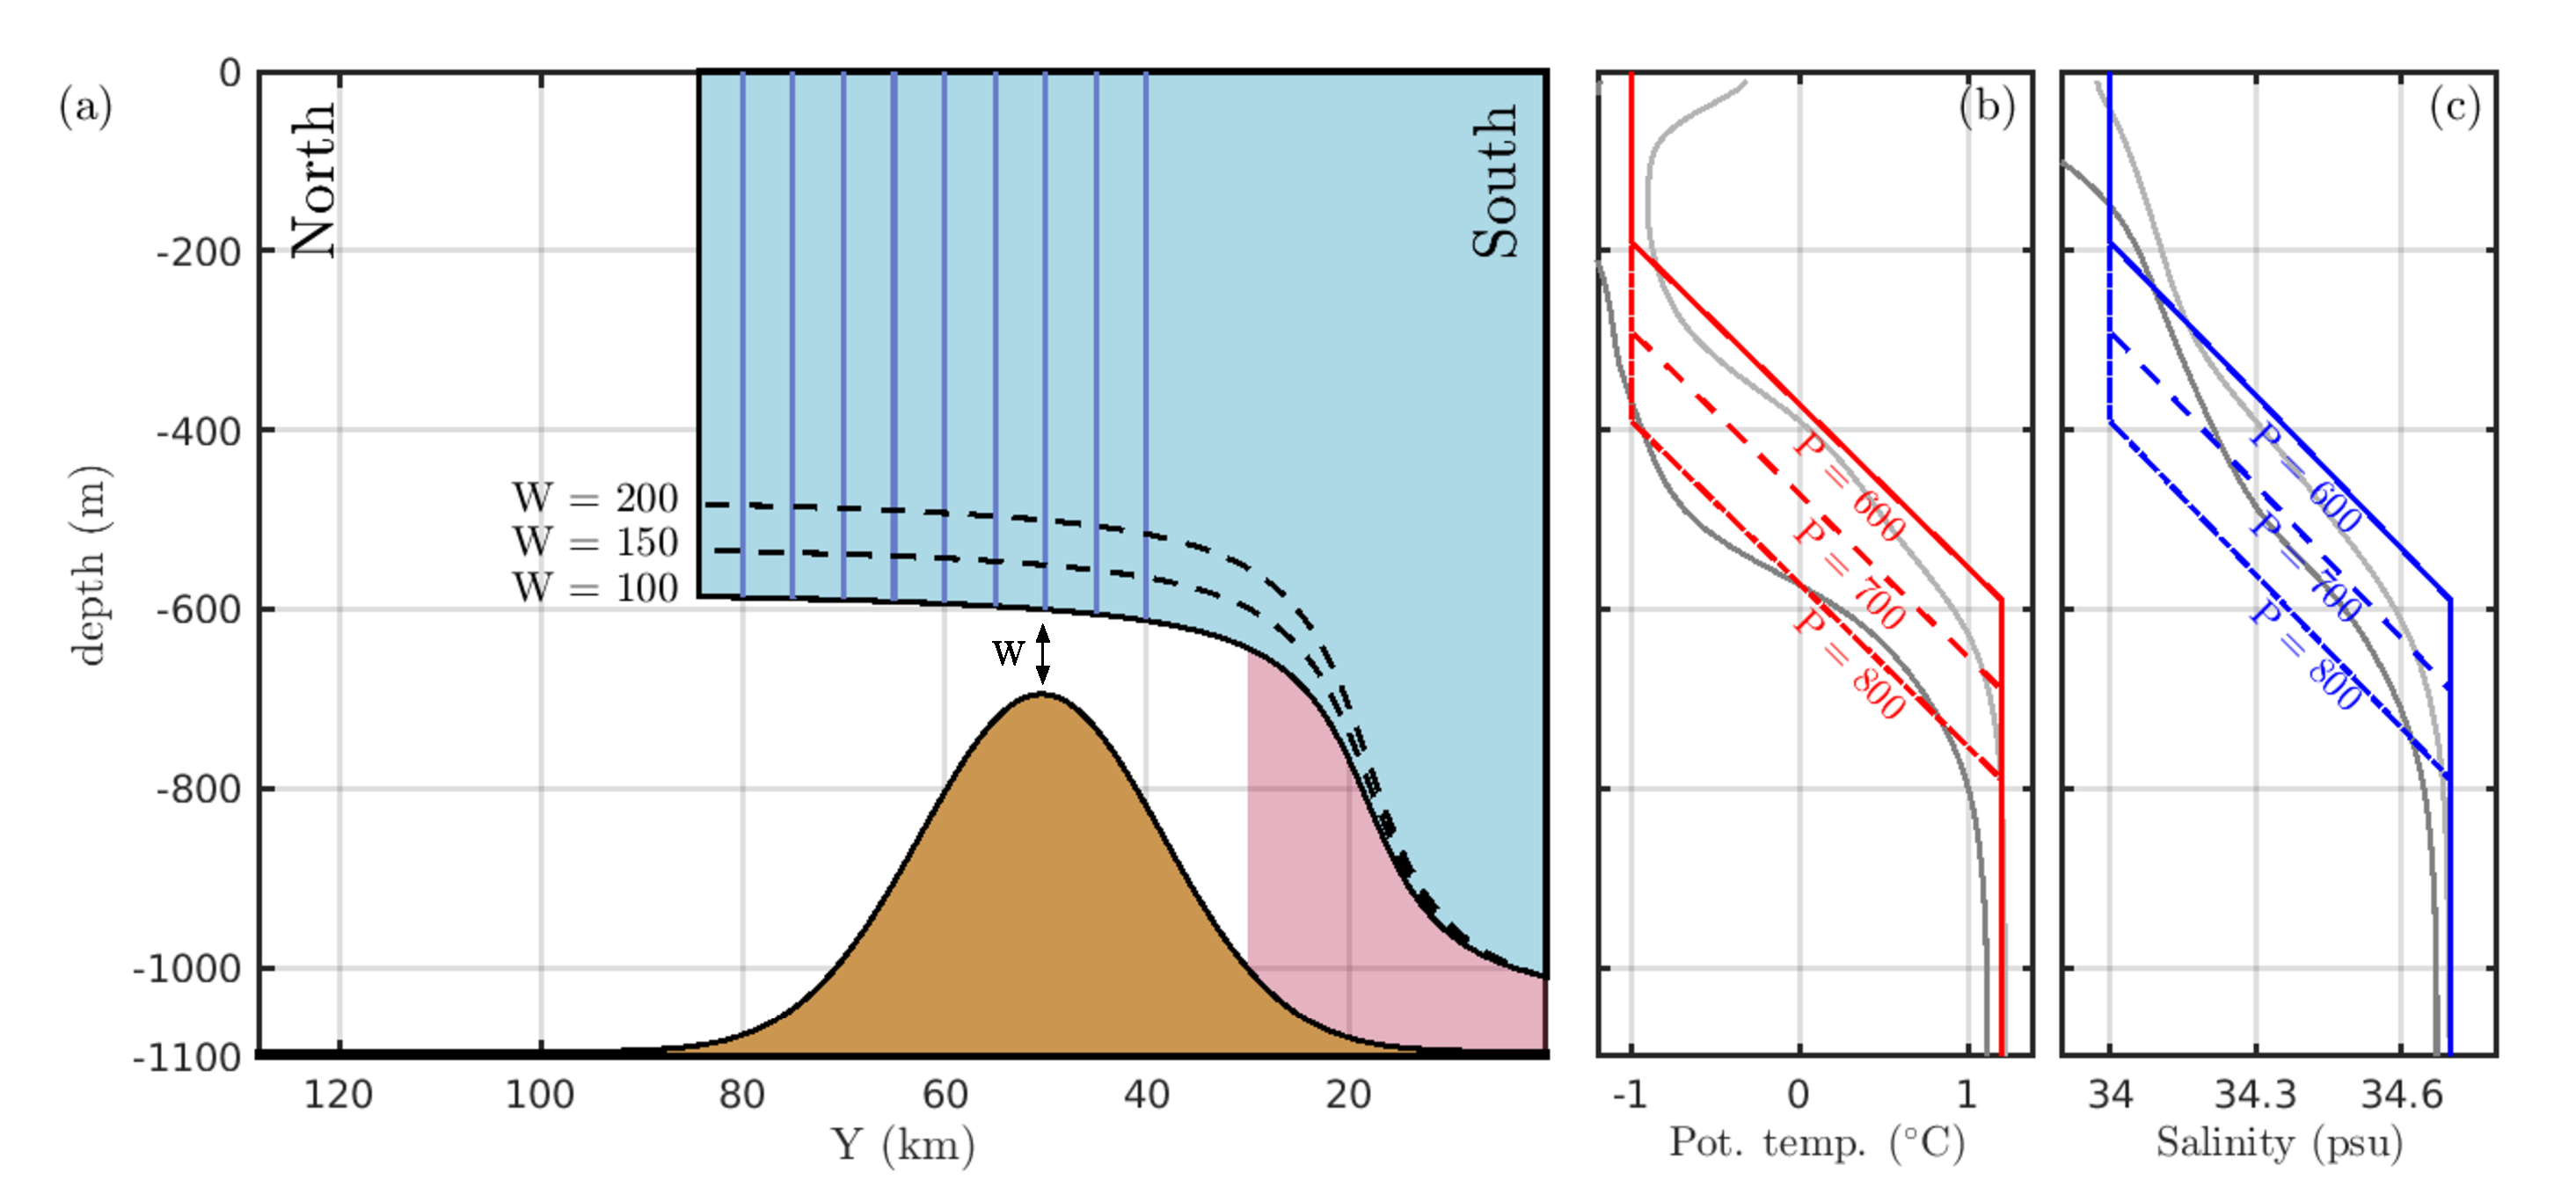
\includegraphics[width = \textwidth]{../make_figures/plots/figure2.pdf}
    \caption{(a) Schematic diagram of the experimental setup. The domain is uniform in the zonal direction (into the page), with extent 48~km. The ocean domain consists of the gridded area, which is bordered by a static ice shelf in $y < 84$~km (shaded blue) and a seabed (shaded brown), which features a prominent ridge. Solid, dashed and dot-dashed black curves indicate the location of the ice shelf base for $W=100$~m, $W=150$~m, and $W=200$~m, respectively, as labelled [the profile of the ice shelf base is defined in equation~\eqref{E:Experiment:Draft}]. Solid blue lines indicate the series of ice front positions considered, which are located at 80, 75, 70, 65, 60, 55, 50, 45, and 40~km offshore of the southern end of the domain at $y = 0~\text{km}$ (the $y$-axis is oriented in this way for consistency with the orientation of PIG in practice, see figure~\ref{fig:figure1}). The shaded red region indicates the inner cavity, defined as the area within 30~km of the southern end of the domain. (b) Temperature and (c) salinity profiles used in the experiments. Different line styles correspond to different values of the pycnocline depth parameter $P$ as follows: $P=600$~m (solid), $P=700$~m (dashed), $P=800$~m (dot-dashed). Light and dark gray lines correspond to temperature and salinity profiles taken from conductivity, temperature, and depth measurements in Pine Island Bay during the austral summers of 2009~\cite{Jacobs2011NatureGeosci} and 2012~\cite{Dutrieux2014Science}, respectively.}
    \label{fig:figure2}
\end{figure}

In this section, we describe the experiments performed in an idealized setup, which we refer to as `idealized experiments'. The idealized experiments have essentially the same setup as~\citeA{DeRydt2014JGeophysResOceans}, albeit it with an updated model configuration, and sections of the ice shelf removed to simulate calving. The domain features a seabed ridge and ice shelf (see figure~\ref{fig:figure2}a), which are both uniform in the zonal direction (and thus so too is the ridge-draft gap between them). In practice, however, the ridge-draft gap is non-uniform (figure~\ref{fig:figure1}c--d); to capture the effect of this variation, we consider the melt response to calving for different thicknesses of the ridge-draft gap. We also consider several different far-field ocean conditions (`hydrographic forcings'): as discussed in \S\ref{S:Introduction}, PIIS melt rates have a sensitive dependence on the hydrographic forcing, via the depth of the pycnocline; we therefore postulate that the melt response to calving might similarly have a sensitive dependence on the hydrographic forcing, and investigate this effect. The role of these idealized experiments, with a highly simplified geometry, is to allow us to isolate the important roles that the thickness of the ridge-draft gap and the hydrographic forcing play in the melt response to calving, as well as elucidate the physical mechanisms responsible for these changes.

We perform a total of 90 idealized experiments, each corresponding to a unique triplet of parameters which describe the thickness of the ridge-draft gap, the hydrographic forcing, and the position of the ice front. These parameters are described in the following two sections. By systematically shifting the ice front towards the (fixed) grounding line between experiments, we simulate calving (and use that name to describe this procedure), but stress that our model includes neither calving dynamics, nor associated processes such as mélange formation. Within each experiment, we solve for the three-dimensional ocean circulation and associated melt rates simultaneously using the Massachusetts Institute of Technology general circulation model (MITgcm)~\cite{Marshall1997JGROceans}. Other than removing sections of the ice shelf, the ice shelf geometry does not change between experiments. Ice shelves themselves enter the ocean model via the exchange of heat and salt at the ice-ocean interface and a steady pressure loading on the ocean surface, i.e. ice dynamics are not taken into consideration when determining the cavity geometry. A steady description of ice shelves is sufficient to assess the response of melt rates to ice shelf calving, which occurs on a timescale much shorter than that on which the ice responds dynamically to perturbations in melting. In the following sections, we provide further details of the ocean model and experimental setup, including the motivation for our choices of parameters.

\subsection{Details of Ocean Model}\label{S:Experiment:Model}
The MITgcm is a z-level general circulation model which includes a partial-cell treatment of topography, allowing an accurate description of both the seabed and ice draft. Our model grid consists of 110 layers with a vertical spacing of $\mathrm{d}z = 10$~m, and a horizontal resolution of $\mathrm{d}x=400$~m. We use the MITgcm in hydrostatic mode with an implicit nonlinear free surface scheme, a third-order direct space-time flux limited advection scheme, and a non-linear equation of state~\cite{Mcdougall2003JAtmosOceanTech}. The Pacanowski-Philander \cite{Pacanowski1981JPhysOcean} scheme parametrizes vertical mixing. Constant values of 15 and 2.5
m\textsuperscript{2} s\textsuperscript{-1} are used for the horizontal Laplacian viscosity and horizontal diffusivity, respectively. The equations are solved on an $f$-plane with $f = -1.4\times10^{-4}~\text{s}^{-1}$.

In each experiment, the simulation is run for twelve months, using a timestep of 30 \si{seconds}. After this spin-up time, the configuration is quasi-steady state. In particular, the field of melt rate is everywhere within 95\% of its final value after three months in each experiment considered here. All results presented here are averaged over the final two months of the simulations.

As mentioned, ice shelves impact on the ocean state via the exchange of heat and salt at the ice-ocean interface. This exchange is described using the so-called `three-equation formulation'~\cite{Holland1999JPhysOcean}, whose implementation in MITgcm has been described thoroughly elsewhere \cite[for example]{Losch2008JGeophysResOceans, DeRydt2014JGeophysResOceans,Dansereau2014JGROceans} and so we do not describe it in detail here. It is useful to note, however, that thermal exchange across the ice-ocean interface is typically dominated by latent heat [over heat conduction into the ice~\cite{Holland1999JPhysOcean}]; in the case of negligible heat conduction, the three-equation formulation for melting reduces to
\begin{linenomath*}
\begin{equation}\label{E:MeltRate}
    \dot{m} = \frac{c_p \gamma_T (T - T_b)}{L},
\end{equation}
\end{linenomath*}
where, $\dot{m}$ is the melt rate. In~\eqref{E:MeltRate}, $T$ is the temperature in the mixed layer adjacent to the ice base, which is considered to have a thickness $\mathrm{d}z$ everywhere, and $T_b$ is the temperature at the ice shelf base, which must be at the local (depth and salinity dependent) freezing point. We refer to the difference of these temperatures, $T- T_b$, as the thermal driving. The quantity $\gamma_t$ is a heat exchange-coefficient, which parametrizes exchange between the mixed layer and the ice shelf base. In our version of the MITgcm, we assume that $\gamma_t$ has a linear dependence of $u^*$, the ocean speed in the viscous boundary layer that forms adjacent to the ice shelf base. We can therefore write
\begin{linenomath*}
\begin{equation}\label{E:MeltRateUdT}
    \dot{m} \propto u^* (T - T_b).
\end{equation}
\end{linenomath*}
We shall return to equation~\eqref{E:MeltRateUdT} when diagnosing the mechanisms responsible for the melt rate response to ice shelf calving.

We use parameter values from \citeA{Holland1999JPhysOcean} in~\eqref{E:MeltRate}--\eqref{E:MeltRateUdT}, except for the drag coefficient in the three-equation formulation of melting, which is set to $4.5\times10^{-3}$. As discussed in \S\ref{S:Realistic}, this value is more appropriate for Pine Island Glacier than the value of $2.5\times10^{-3}$ suggested by \citeA{Holland1999JPhysOcean}.

\subsection{Ice Shelf Geometry and Seabed Bathymetry}\label{S:Experiment:Geometry}
The geometry of the idealized setup is shown schematically in figure~\ref{fig:figure2}a. It is uniform in the zonal direction, along which the $x$-axis is aligned, and the $y$-axis is aligned along the meridional direction. Note that although PIG is aligned approximately east-west, we orient this idealized model north-south, as is standard~\cite{Grosfeld1997JGROceans, DeRydt2014JGeophysResOceans} and results are independent of this choice of orientation.

The seabed has a shifted Gaussian profile,
\begin{linenomath*}
\begin{equation}\label{E:Experiment:Bed}
    b(x,y) = -1100 + 400 \exp\left[-\frac{\left(y - 50\times 10^3\right)^2}{2\sigma^2}\right],
\end{equation}
\end{linenomath*}
where $\sigma = 12$~km is the length scale over which this profile decays towards zero. The profile~\eqref{E:Experiment:Bed} corresponds to a ridge that peaks at a height of 400~m above the surrounding bathymetry. This peak occurs 50 km from the southern end of the domain at $y=0$~km, which we consider to be the grounding line (figure~\ref{fig:figure2}a).

In reality, the variability in both PIIS draft and the height of the seabed ridge result in a ridge-draft gap that varies between approximately 100 m at its thinnest, to greater than 300 m at its thickest (figure~\ref{fig:figure1}c--d). Since we use the same, zonally uniform, seabed geometry (and, in particular, the same ridge height) in all of our idealized experiments, we aim to gain insight into the effect of variation in the ridge-draft gap by considering several different values of $W$ -- the vertical distance between the crest of the seabed ridge and the ice shelf base (figure~\ref{fig:figure2}a). In our setup, $W$ enters the model only via the ice profile; following~\citeA{DeRydt2014JGeophysResOceans}, we use an ice shelf draft given by
\begin{linenomath*}
\begin{equation}\label{E:Experiment:Draft}
    H(y) = \begin{cases}
    \left(\frac{310 + W}{2.64}\right)\tan^{-1}\left(\frac{y}{5882} -3\right) & \text{for}~y < y_f,\\
    0  & \text{for}~y \geq y_f.
    \end{cases}
\end{equation}
\end{linenomath*}
Here $y_f$ is the variable location of the ice front (see below). We stress that the ice draft profile~\eqref{E:Experiment:Draft} is not obtained from ice dynamics considerations, but selected for its qualitative similarity to PIIS: it includes a flatter section offshore of the ridge and a steeper section inshore of the ridge, thus resembling variations in the basal slope that have been inferred from radar and satellite data. Note that the combination of the bathymetry~\eqref{E:Experiment:Bed} and ice shelf draft~\eqref{E:Experiment:Draft} means that the water column thickness is small, but nonzero at the grounding line (figure~\ref{fig:figure2}a); this is because the MITgcm requires at least two grid cells in the vertical direction to permit horizontal transfer.

We consider three different values of $W$ here: $W=100$~m, $W=150$~m, and $W=200$~m. The smallest value, $W=100$~m, corresponds to the minimum observed ridge-draft gap under PIIS (figure~\ref{fig:figure1}d), while the largest value, $W=200$~m, corresponds to an upper bound, above which there is little melt response to calving, as we shall see.

As mentioned, the front position $y_f$ is systematically reduced between experiments to simulate calving. We consider a total of ten different ice front positions, using $y_f=84$, $80$, $75$, $70$, $65$, $60$, $55$, $50$, $45$, and $40~\text{km}$, which correspond to calved lengths of $l_c=0$, $4$, $9$, $14$, $19$, $24$, $29$, $34$, $39$, and $44~\text{km}$, respectively. Those experiments with $l_c = 0$~km are referred to as `uncalved' experiments, serving as a benchmark against which results for $l_c >0$~km are compared. There are both pragmatic and physical reasons for choosing this particular range of values for $l_c$: the setup with $\ell_c = 0$~km has an ice shelf whose length is approximately equal to the observed distance of the ice front from the PIG grounding line in 2009, before significant calving took place in the late 2010s; the largest value, $l_c = 44~\text{km}$, is chosen as a compromise between allowing us to consider scenarios in which the ice front has been retreated significantly beyond the ridge, whilst retaining a large area that is shared by each experiment (as we discuss further in \S\ref{S:Baseline}, the area over which melt rates are averaged must be invariant to calving for a robust assessment of the melt response to calving).

\subsection{Hydrographic Forcing}\label{S:Experiment:Hydrography}
For each unique value of $W$ and $l_c$, we perform three experiments, each with a different hydrographic forcing. The range of these hydrographic forcings covers that which is observed in practice (see below). Comparing the results of these experiments gives us an indication of the sensitivity of our results to hydrographic forcing. 

The hydrographic forcing is imposed on the model by means of a restoring boundary condition at the northern end of the domain ($y = 128$~km in figure~\ref{fig:figure2}a): at this boundary, the temperature and salinity are restored to specified vertical profiles, shown in figure~\ref{fig:figure2}b and c, respectively, over a distance of five horizontal grid cells (total length 2 km) with a restoring timescale that varies from 12~hours at the boundary to 60~hours in the interior.  The specified temperature and salinity profiles are piecewise linear functions of depth: they are constant in both an upper (temperature $-1^\circ$C, salinity $34$~PSU) and lower layer (temperature $1.2^\circ$C, salinity $34.7$~PSU), and these layers are separated by a pycnocline of 400~m thickness, across which the temperature and salinity vary linearly. The pycnocline begins at a variable depth $P$ (a higher $P$ corresponds to a deeper pycnocline), which parametrizes the entirety of the temperature and salinity profiles (figure~\ref{fig:figure2}b, c); the three hydrographic forcings we consider have $P=600$ m, 700 m, and 800 m.

%why do we choose these conditions
These piecewise linear profiles are approximations to typical conditions for PIB \cite{Jacobs1996GRL, Dutrieux2014Science, Jenkins2018NatureGeo} (figure~\ref{fig:figure2}b--c). As mentioned, the record of hydrographic conditions in PIB has revealed significant variability in the depth of the pycnocline on interannual timescales~\cite{Dutrieux2014Science}; the profiles with $P=600$~m and $P=800$~m are approximations to profiles observed in PIB in the years 2009 and 2012, respectively (figure~\ref{fig:figure2}b, c). These two years approximately span the range of observed conditions: in 2009, the average depth of the pycnocline was at its shallowest level on record, while in 2012 the average depth of the pycnocline was at its second-deepest level on record~\cite{Webber2017NatureComms}.

%wrap up the experiments:
In summary, we perform a total of 90 idealized experiments. Each is uniquely identified by a $(W,~P,~l_c)$ triplet, where $W$ $\in \{100,~150,~200\}~\text{m}$, $P$ $\in \{600, 700, 800\}~\text{m}$, and $l_c \in \left\{0,~4,~9,~14,~19,~24,~29,~34,~39,~44\right\}~\text{km}$. We consider the experiment with $W=100$~m, $P=600$~m, and $l_c=0$~km to be the baseline; this corresponds to the extreme scenario with the narrowest ridge-draft gap (the strongest topographic barrier), the hydrographic forcing with the shallowest pycnocline (thickest CDW layer), and an uncalved ice shelf. In the following section, we describe the results of the baseline experiment. In \S\ref{S:Results:lc}, we describe the results of applying the calving perturbation to the baseline, presenting results of those experiments with  $W=100~\text{m},~P=600~\text{m},~l_c>0~\text{km}$; i.e. we describe the melt response to calving for $W=100~\text{m}$, $P = 600~\text{m}$. In \S\ref{S:Results:H} and~\ref{S:Results:P}, we respectively describe how the melt response to calving changes for the different values of $W$ and $P$ considered here.

\section{Results for the Baseline Experiment ($W=100$~m, $P=600$~m, $\ell_c = 0$~km)}\label{S:Baseline}
In this section, we describe the results for the baseline experiment with $W=100~\text{m}$, $P=600~\text{m}$, which correspond to the solid lines in figure~\ref{fig:figure2}, and $l_c=0~\text{km}$. %introduce the idea of the inner cavity, why do we use this metric
Before we proceed, we introduce the `inner cavity' -- the area of the ocean domain that is located within 30~km of the southern boundary (indicated by the red-shaded region in figure~\ref{fig:figure2}a). We use the mean melt rate in the inner cavity, referred to henceforth as the `inner cavity melt rate', as a single metric to quantify changes in melt rate with calving. Since the melt rate is highly spatially variable (see below) it is necessary to consider a fixed area that is common to each experiment when assessing changes in melt rate with calving. Indeed, averaging over the whole shelf, for example, would make smaller shelves appear to have anomalously large melt rates, since the region of high melt close to the grounding line would occupy a greater proportion of the entire shelf. Our choice of 30~km in this definition reflects a compromise between enabling simulations in which the ice front is retreated a significant distance beyond the ridge to be included (the smallest shelf we consider must be larger than the inner cavity, if the entirety of the inner cavity is to be included in each experiment), and considering a reasonably large section of the uncalved ice shelf over which the melt rate is averaged. Crucially, this choice includes the region adjacent to the grounding line, where changes in melt rate are particularly important for the dynamics of the grounded ice sheet \cite{Seroussi2014Cryo, Athern2017GRL}. Although the absolute values of the inner cavity melt rate \textit{are} dependent on the length of region chosen in its definition, we verified that the trends and key results presented here are independent of this choice.

\begin{figure}
    \centering
    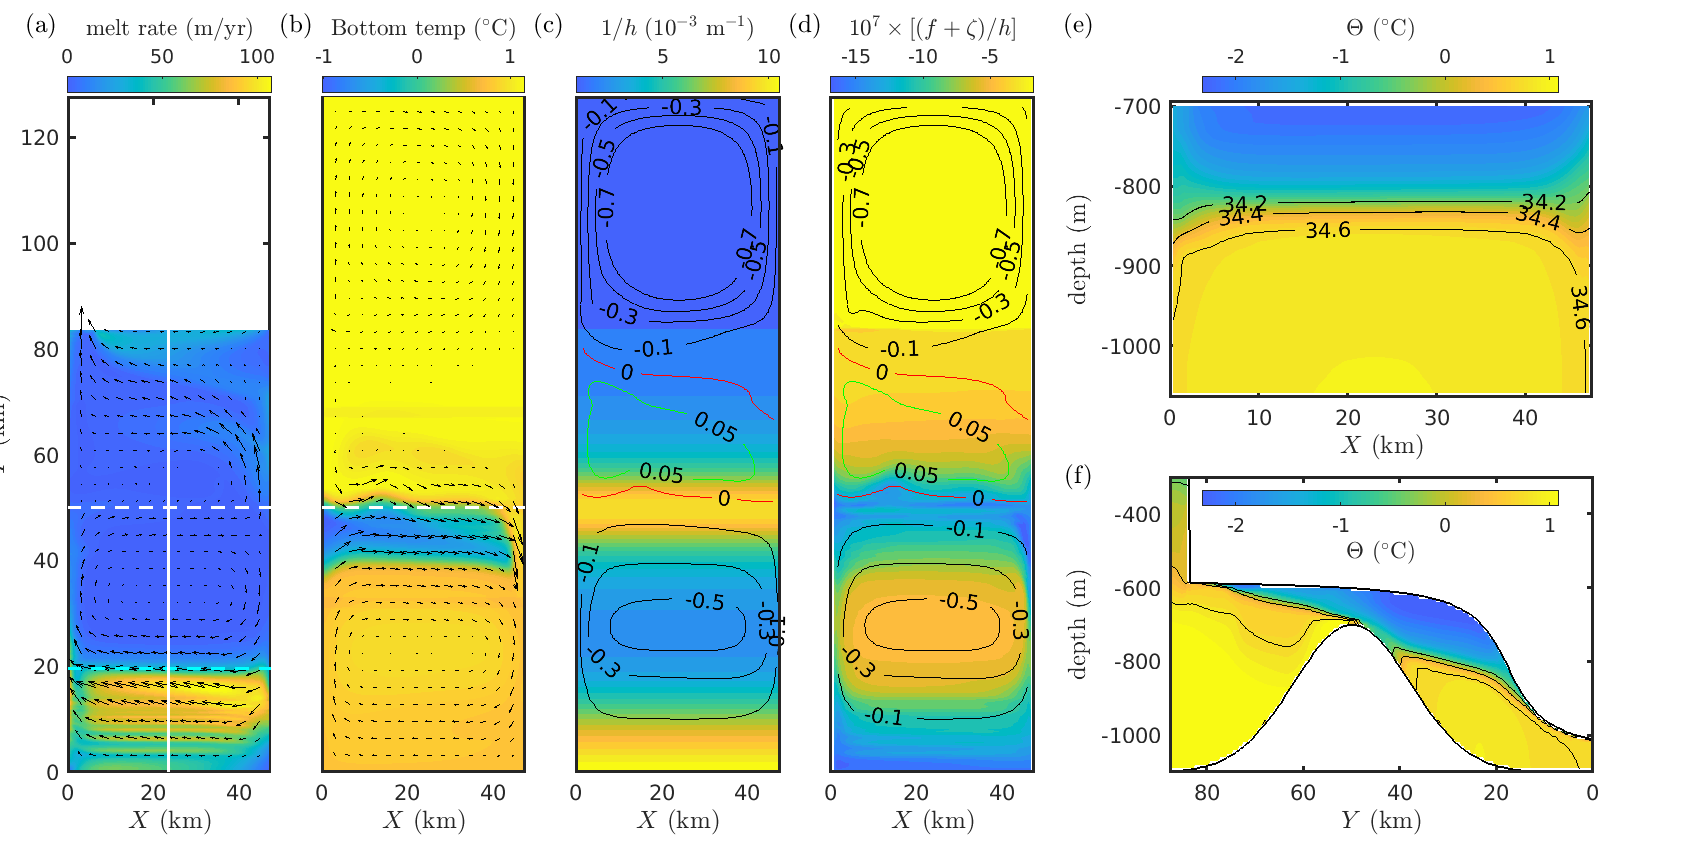
\includegraphics[width = \textwidth]{../make_figures/plots/figure3.png}
    \caption{Ice-ocean properties that characterize the baseline experiment, with $W = 100$~m, $P = 600$~m, and $\ell_c = 0$~km. (a) Melt rate (colors) and ocean velocities (arrows, every fifth velocity vector is plotted), averaged over the three grid cells adjacent to the ice-ocean interface. White areas correspond to open ocean. The white dashed line indicates the location of the ridge crest; the white solid line indicates $y=20~\text{km}$, along which the section in (e) is taken; and the magenta dashed line indicates the center line $x = 24~\text{km}$, along which the section in (f) is taken. (b) Ocean temperature (colors) and velocity (arrows) averaged over the three grid cells closest to the seabed. The scale bar for velocity vectors in (a) is also appropriate for (b). (c) Inverse water column thickness $1/h$  and (d) barotropic potential vorticity (colors) alongside barotropic stream function (contours, in units of Sv) at levels 0.05 (green) 0 (red), -0.1, -0.3, -0.5, and -0.7~Sv (all black). (e) Zonal cross-section taken at $y=20~\text{km}$ up to the ice shelf base, showing potential temperature (colors) and salinity contours at the 34.2, 34.4, and 34.6~PSU levels, as indicated. (f) Meridional cross-section of temperature and salinity [with colors and contours as in (d)], taken along the centerline $x = 24$~km.}
    \label{fig:figure3}
\end{figure}

%describe each of what we see: melt rate, general observations
Ice-ocean properties that characterize the baseline simulation are shown in figure~\ref{fig:figure3}. Melt rates (figure~\ref{fig:figure3}a) are below  20~m~year\textsuperscript{-1} everywhere, except for a region located within 20~km of the grounding line, where the melt rate reaches a maximum of 120~m~year\textsuperscript{-1}. The average melt rate over the whole shelf is approximately 20~m~year\textsuperscript{-1}.  While this is lower than the value of 33$\pm$2~m~year\textsuperscript{-1} that was estimated by~\citeA{Jenkins2010NatureGeo} based on observations in PIB in 2009, to which the $P=600$~m case corresponds, this discrepancy is in the expected direction: the baseline simulation corresponds to the extreme scenario in which the ridge-draft gap is set everywhere to the minimum gap that is observed in practice, impeding the supply of warm water across the ridge. The melt rate is proportional to the product of the ice-ocean mixed layer circulation and thermal driving [see equation~\eqref{E:MeltRateUdT}]; while the circulation is vigorous everywhere inshore of the ridge, high melt rates are restricted to the area south of $y=20$~km: to the north of $y=20$~km, a cold and fresh meltwater plume sits adjacent to the ice-ocean interface (figure~\ref{fig:figure3}e) and the temperature difference between the ocean and ice base is therefore much smaller than to the south of $y=20$~km, where the ice is adjacent to warm water.

%why does the melt rate look like it does
%\red{Does this paragraph add anything? Bit more detail on the melt pattern?} The melt rate is proportional to the product of the ice-ocean mixed layer circulation and thermal driving [see equation~\eqref{E:MeltRateUdT}]. \blue{On the scale of the entire cavity,}\rout{Cavity} circulation (figure~\ref{fig:figure3}a--d) is characterized by a geostrophic cyclonic circulation. South of the seabed ridge, this circulation is directed northward at the western boundary ($x=0$~km) and southward at the eastern boundary ($x=48$~km). While the circulation is vigorous everywhere inshore of the ridge, high melt rates are restricted to the area south of $y=20$~km: to the north of $y=20$~km, a cold and fresh meltwater plume sits adjacent to the ice-ocean interface (figure~\ref{fig:figure3}e) and the temperature difference between the ocean and ice base is therefore much smaller than to the south of $y=20$~km, where the ice is adjacent to warm water.

%we can use the bsf
When the ice shelf is calved in the subsequent simulations, the only a priori imposed change on the experiment is the water column thickness in those regions of the domain in which the ice shelf is removed (the resulting buoyancy forcing also changes, but this emerges from the simulation a posteriori). It is therefore instructive to consider the effect of changes in water column thickness, which influence the flow only through barotropic dynamics; we shall therefore use a primarily barotropic framework to diagnose the melt response to calving. 

Barotropic velocities $\hat{\mathbf{u}} = (\hat{u}, \hat{v})$ must satisfy the barotropic potential vorticity (BPV) equation [see~\citeA{Patmore2019JPO}, for example]:
\begin{linenomath*}
 \begin{align}
 \frac{\nu}{h}\nabla^2 \zeta + \frac{1}{\rho_0 h}\mathbf{k} . \nabla \times \left( \frac{\mathbf{\tau}_w - \mathbf{\tau}_b}{h}\right) &= \frac{\mathrm{D}}{\mathrm{D}t}\left( \frac{f + \zeta}{h}\right) \label{E:BPVeq} \\ &\approx  \hat{v} f  \frac{\mathrm{d}}{\mathrm{d}y} \left(\frac{1}{h}\right) + \hat{\mathbf{u}}.\nabla \left(\frac{\zeta}{h}\right) \label{E:BPVeq2}
 \end{align}
 \end{linenomath*}

where $h = h(y)$ is the water column thickness, $\zeta = \partial \hat{v} / \partial x - \partial \hat{u} / \partial y$ is the relative vorticity,  $\nu$ is the kinematic viscosity, $\rho_0$ is a reference density, $\mathbf{\tau}_w$ is the surface stress, $\mathbf{\tau}_b$ is the bottom stress, and $\mathbf{k}$ is the unit vector pointing in the upwards vertical. We collectively refer to the terms on the left-hand side of~\eqref{E:BPVeq} as viscous sources of BPV, and the first and second terms on the right-hand side of~\eqref{E:BPVeq2} as planetary and relative sources of BPV, respectively. In~\eqref{E:BPVeq}--\eqref{E:BPVeq2}, $f = 2\Omega \sin \theta$ is the Coriolis frequency, where $\Omega = 7.2921\times10^{-5}$ is the rotation rate of the Earth and $\theta$ is the longitude. In practice, the relatively small size of the idealized domain means that $\theta$, and thus $f$, can be assumed constant.  The approximation~\eqref{E:BPVeq2} results from this assumption, alongside that of a zonally uniform water column thickness, and steady state conditions.

Equation~\eqref{E:BPVeq} implies that in steady, inviscid flow with no bottom or surface stress, a water column advected by the flow will conserve its barotropic potential vorticity (BPV), $(f + \zeta)/h$. In our idealized domain, water column thickness is uniform in the zonal direction, i.e. $h$ varies only in the meridional direction (figure~\ref{fig:figure3}c). As flow travels in the meridional direction, it crosses $1/h$ contours, so another source is required to balance the resulting BPV production. This can be achieved by adjusting relative vorticity, $\zeta$, but in places where that balance cannot hold, viscous stresses intervene to complete the BPV balance. Plots of $1/h$ (figure~\ref{fig:figure3}c), $(f + \zeta)/h$ (figure~\ref{fig:figure3}d), and the barotropic stream function (figure~\ref{fig:figure3}c, d) allow us to determine where in our domain each of the terms in equation~\eqref{E:BPVeq} play an important role. In regions where barotropic streamlines follow east-west aligned contours of constant water column thickness (figure~\ref{fig:figure3}c), relative and viscous sources of vorticity are small; where contours of constant BPV (colors in figure~\ref{fig:figure3}d) deviate from these east-west aligned $f/h$ contours, relative vorticity plays an important role; finally, viscous stresses play an important role where barotropic streamlines (lines in figure~\ref{fig:figure3}d) deviate from contours of constant BPV (colors in figure~\ref{fig:figure3}d).

The ice front and the seabed ridge are the two predominant discontinuities in the water column thickness, and therefore act as BPV barriers: in order to cross these features in a meridional direction, barotropic flow must either change its relative vorticity or be subject to viscous stresses. These BPV barriers divide the domain up into three regions: inshore of the ridge, offshore of the ridge (but under the ice shelf, referred to as the `outer cavity'), and the open ocean. 

%what happens in the outer cavity
In the open ocean, the combination of boundary restoring to salty water at the region's northern boundary and ice shelf freshwater influx at its southern boundary tilts the isopycnals, resulting in a cyclonic circulation. Note that, except for in the vicinity of the ice front, the gyre in the outer region has uniformly spaced streamlines (figure~\ref{fig:figure3}c): the flow is not faster along the lateral boundaries than it is on the north and south boundaries. This corresponds to a uniform the relative vorticity, which is consistent with the approximately constant water column thickness in the interior of this region. At the ice front, there is a vertical wall. In any flow crossing this wall, relative vorticity cannot balance the planetary BPV source (the flow cannot gain or lose vorticity over a zero length scale). Instead, the requirement for sudden shear causes viscous terms (left-hand side of~\eqref{E:BPVeq}) to arise: the flow uses viscous sources to balance the planetary vorticity source as it crosses the ice front (seen as deviations between colors and contours in figure~\ref{fig:figure3}d). In the simulations, the gyre in the open ocean spins up until the shear at the ice front generates enough viscosity to permit barotropic flow to cross the ice front. This allows the heat flux, which causes melting thus tilting the isopycnals, to be maintained.


%what happens in the inner cavity 
For the same reasons as in the open ocean (boundary restoring versus ice shelf freshwater flux), the barotropic dynamics inshore of the ridge are also dominated by a large cyclonic gyre. It is interesting to note, however, that the circulation in this region is subtly different from the open ocean. This is ultimately because north-south flow in the inner cavity requires contours of constant water column thickness to be crossed: a source of BPV is required to balance the associated planetary vorticity source. To see this, consider the south-west quadrant of the inner cavity: when the flow is northward, into a thicker water column, the planetary source term is positive ($f<0$, $\hat{v}>0$, $\mathrm{d}(1/h)/\mathrm{d}y<0$); one way in which a relative vorticity source can balance this with a negative value is if the flow gains cyclonic (negative) vorticity ($\hat{v}>0$, $\partial \zeta/\partial y<0$). This can be extended to the other quadrants: if the flow is heading southwards, then the sign of these terms switches, and if the flow is heading into a thinner water column, they switch again. In response, the relative vorticity becomes more negative in the south-west and north-east quadrants, and less negative in the north-west and south-east quadrants. These changes explain why the flow is intensified on the eastern and western boundaries: the flow must intensify (streamlines converge) to produce the required relative vorticity changes, i.e. the meridional topography variation is concomitant with zonal intensification of the meridional flow.

%what happens in the dead region...
The outer cavity sits between the two regions hosting strongly topographically constrained circulations to its north and south. There is little flow in this region: the anti-cyclonic circulation that forms there (figure~\ref{fig:figure3}c) is much weaker than that in the open ocean or inshore of the ridge. This flow is not strong enough to generate the shear, and thus vorticity, that would be required at the ridge crest to balance planetary vorticity in southward flow across it (note the zero barotropic contour at the ridge crest, figure~\ref{fig:figure3}b). Just offshore of the ridge, flow is directed eastwards, parallel to the ridge crest. Where this jet meets the eastern domain boundary, the baroclinic component of flow provides the region inshore of the ridge with warm water from offshore of the ridge (figure~\ref{fig:figure3}b). However, the total flux across the ridge provided by this baroclinic flow (approximately 0.01~Sv) is small in comparison with the typical barotropic fluxes in the cavity, which are on the order of 0.3~Sv  (figure~\ref{fig:figure3}c), i.e. the boundary current flushing of the inner cavity is relatively weak in comparison with the inner cavity circulation.

In the absence of significant flow across the ridge, the inshore side of the ridge hosts meltwater, which is recirculated rather than flushed out. Warm water entering the region inshore of the ridge at the eastern boundary mixes with this meltwater as it crosses the ridge, causing it to be lightly modified and resulting in a bottom temperature that is slightly cooler (approximately 0.8${}^\circ$C) inshore of the ridge than offshore (approximately 1.3${}^\circ$C, see figure~\ref{fig:figure3}b,~e).

% As mentioned, the total flux of warm water over the ridge is relatively small and a relatively strong circulation in the inner cavity is therefore required to generate the melt required to provide the buoyancy forcing that balances boundary restoring at the northern end of the domain.

In summary, in the baseline simulation, which has a strong BPV barrier restricting CDW access to the inner cavity, strong cyclonic gyres are spun up in the open ocean and in the region inshore of the ridge, while in the outer cavity, the circulation is weak. The two cyclonic gyres are dynamically disconnected from one another, and barotropic flow is unable to cross the ridge. A baroclinic current at the eastern boundary of the ridge crest provides a modest source of lightly modified CDW, and thus heat for melting, to the region inshore of the ridge. The hosting of cold meltwater on the ice-ocean interface inshore of the ridge means that high melt rates are restricted to a region just downstream of the grounding line. 

\section{Melt Response to Calving}\label{S:Results:lc}
In this section, we describe how, and why, the inner cavity melt rate responds when the ice shelf is sequentially calved from the baseline configuration. The inner cavity melt rate as a function of the calved length $l_c$ is shown in figure~\ref{fig:figure4}a. We see that, while the ice shelf front is located far offshore of the ridge ($l_c< 14$~km), removing sections of ice results in only a weak increase in the inner cavity melt rate. However, as the ice shelf front is retreated further towards the ridge, the melt rate increases more strongly with calving, reaching a maximum of 73~m~year\textsuperscript{-1} (70\% larger than in the baseline simulation) when the ice shelf is located approximately 5~km north of the ridge crest. Perhaps surprisingly, retreating the ice front slightly further to sit directly above the ridge crest results in a significant decrease in the inner cavity melt rate of approximately 15\% (from 73~m~year\textsuperscript{-1} to 64~m~year\textsuperscript{-1}). Finally, the inner cavity melt rate is approximately independent of ice front position when the ice front is located inshore of the ridge ($l_c>34$~km).

%figure 5: (a) plot of mean melt rate as a function of extent and (b) millgate decomposition
\begin{figure}
    \centering
    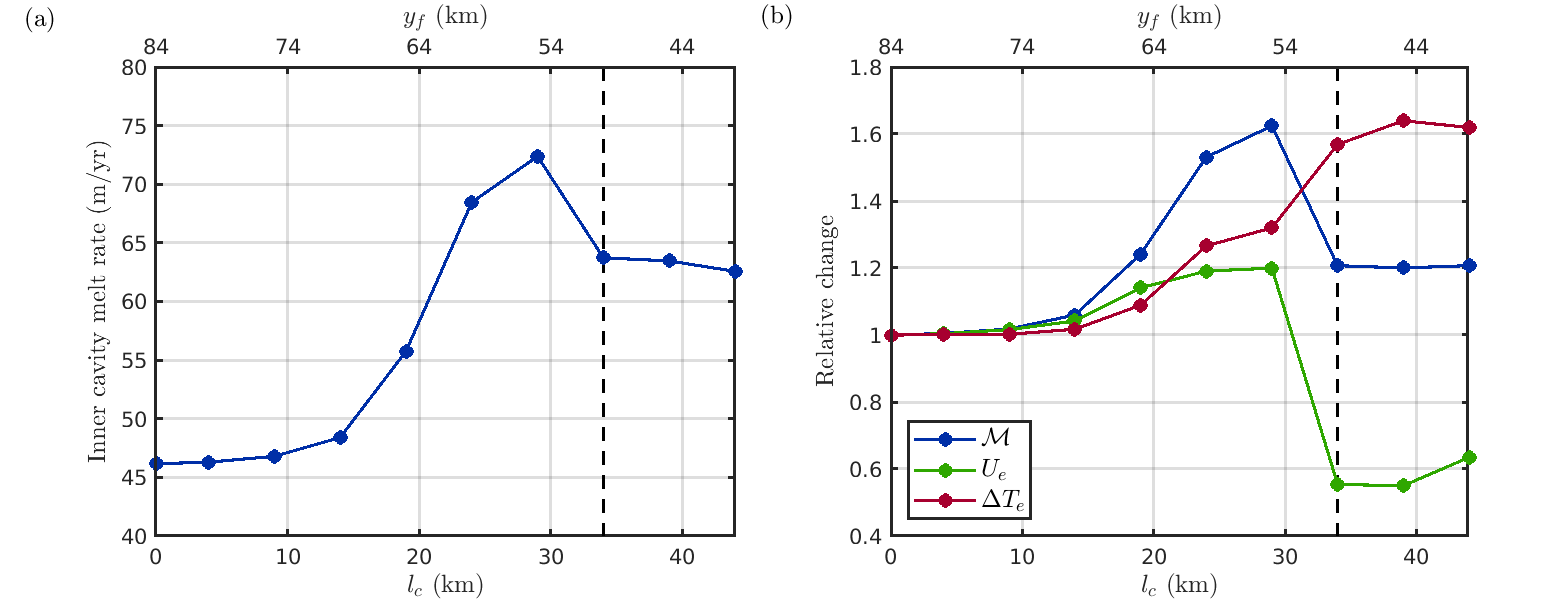
\includegraphics[width = \textwidth]{../make_figures/plots/figure4.png}
    \caption{(a) Mean inner cavity melt rate as a function of the calved length $l_c$. The black dashed line indicates the position of the ice front when it is located directly above the seabed ridge. (b) Velocity-thermal driving decomposition: decomposition of changes in inner cavity melt rate relative to the baseline simulation into changes associated with boundary layer speed $U_e$ [green curve, equation~\eqref{E:MillgateDecompU}] and thermal driving $\Delta T_e$ [red curve, equation~\eqref{E:MillgateDecompDT}]. The blue curve indicates the change in melting relative to the uncalved simulation [equation~\eqref{E:MillgateDecompMelt}]. The green dashed line indicates the barotropic velocity effect $U_{be}$ [equation~\eqref{E:MillgateDecompUbaro}].  }
    \label{fig:figure4}
\end{figure}

%explain what the Millgate decomposition.
To understand the reasons for this melt response to calving, it is instructive to return to equation~\eqref{E:MeltRateUdT}, which indicates that the melt rate is proportional to the product of the boundary layer velocity and thermal driving. To investigate the relative roles of variations in both of these quantities in the changes to the inner cavity melt rate, we compute~\cite{Millgate2013JGROceans}
\begin{linenomath*}
\begin{align}
  U_{e}(l_c) &=  \frac{\int_{\text{IC}}~u^*(x,y; l_c)~\Delta T(x,y;l_c = 0)~\mathrm{d}x\mathrm{d}y}{\int_{\text{IC}}~ u^*(x,y; l_c = 0)~\Delta T(x,y;l_c = 0)~\mathrm{d}x\mathrm{d}y}, \label{E:MillgateDecompU}\\ \Delta T_{e}(l_c) &=  \frac{\int_{\text{IC}}~u^*(x,y; l_c=0)~\Delta T(x,y;l_c)~\mathrm{d}x\mathrm{d}y}{\int_{\text{IC}}~ u^*(x,y; l_c = 0)~\Delta T(x,y;l_c = 0)~\mathrm{d}x\mathrm{d}y}, \label{E:MillgateDecompDT}
\end{align}
\end{linenomath*}
where `IC' refers to the inner cavity. Recall that $u^*(x,y;l_c)$ and $\Delta T(x,y;\ell_c)$ are the boundary layer velocity and thermal driving, respectively, that emerge from the experiment in which the ice front is located at $y = l_c$. The quantities in~\eqref{E:MillgateDecompU}--\eqref{E:MillgateDecompDT} are compared, for a given calved length $l_c$, to the relative change in melting over the baseline simulation,
\begin{linenomath*}
 \begin{equation}\label{E:MillgateDecompMelt}
   \mathcal{M}(l_c) =  \frac{\int_{\text{IC}}~u^*(x,y; l_c)~\Delta T(x,y;l_c)~\mathrm{d}x\mathrm{d}y}{\int_{\text{IC}}~ u^*(x,y; l_c = 0)~\Delta T(x,y;l_c = 0)~\mathrm{d}x\mathrm{d}y}.
 \end{equation}
 \end{linenomath*}

The quantities~\eqref{E:MillgateDecompU}--\eqref{E:MillgateDecompMelt} are plotted in figure~\ref{fig:figure4}b as a function of $l_c$.  Here, a melt response to calving that results exclusively from changes in thermal driving would be indicated by indistinguishable blue and red curves, and a green curve that takes the value unity for all $\ell_c$;  a melt response that results exclusively from changes in boundary layer velocity would be indicated by indistinguishable blue and green curves, and a red curve that takes the value unity for all $\ell_c$. Henceforth, we refer to this comparison as a `velocity-thermal driving decomposition'. %(Note, however, that while the relative change in melt rate depends on the changes in velocity and thermal driving, this relationship is not linear.)

%what do these plots tell us about what is responsible for the changes?
The velocity-thermal driving decomposition (figure~\ref{fig:figure4}b) indicates that both changes in the boundary layer velocity and thermal driving play an important role in the melt response to calving, i.e. neither plays a dominant role.  When the ice front is located offshore of the ridge ($l_c < 30$~km), ice front retreat results in increases in both the boundary layer velocity and thermal driving: these increases are complementary, acting in unison to increase the inner cavity melt rate as calving proceeds. When the calving front is retreated to sit above the ridge, the thermal driving effect increases further, while the velocity effect decreases sharply, corresponding to a significant reduction in the boundary layer velocity at this point. This reduction in cavity circulation outweighs the increase in thermal driving, leading to an overall reduction in the inner cavity melt rate. When the ice shelf is calved further beyond the ridge, both the thermal driving and boundary layer velocity effects are approximately constant.

%figure 6:  (a) row of melt rate (colours) and BSF contours, (b) zonal sections, (c,d) meridional sections
\begin{figure}
    \centering
    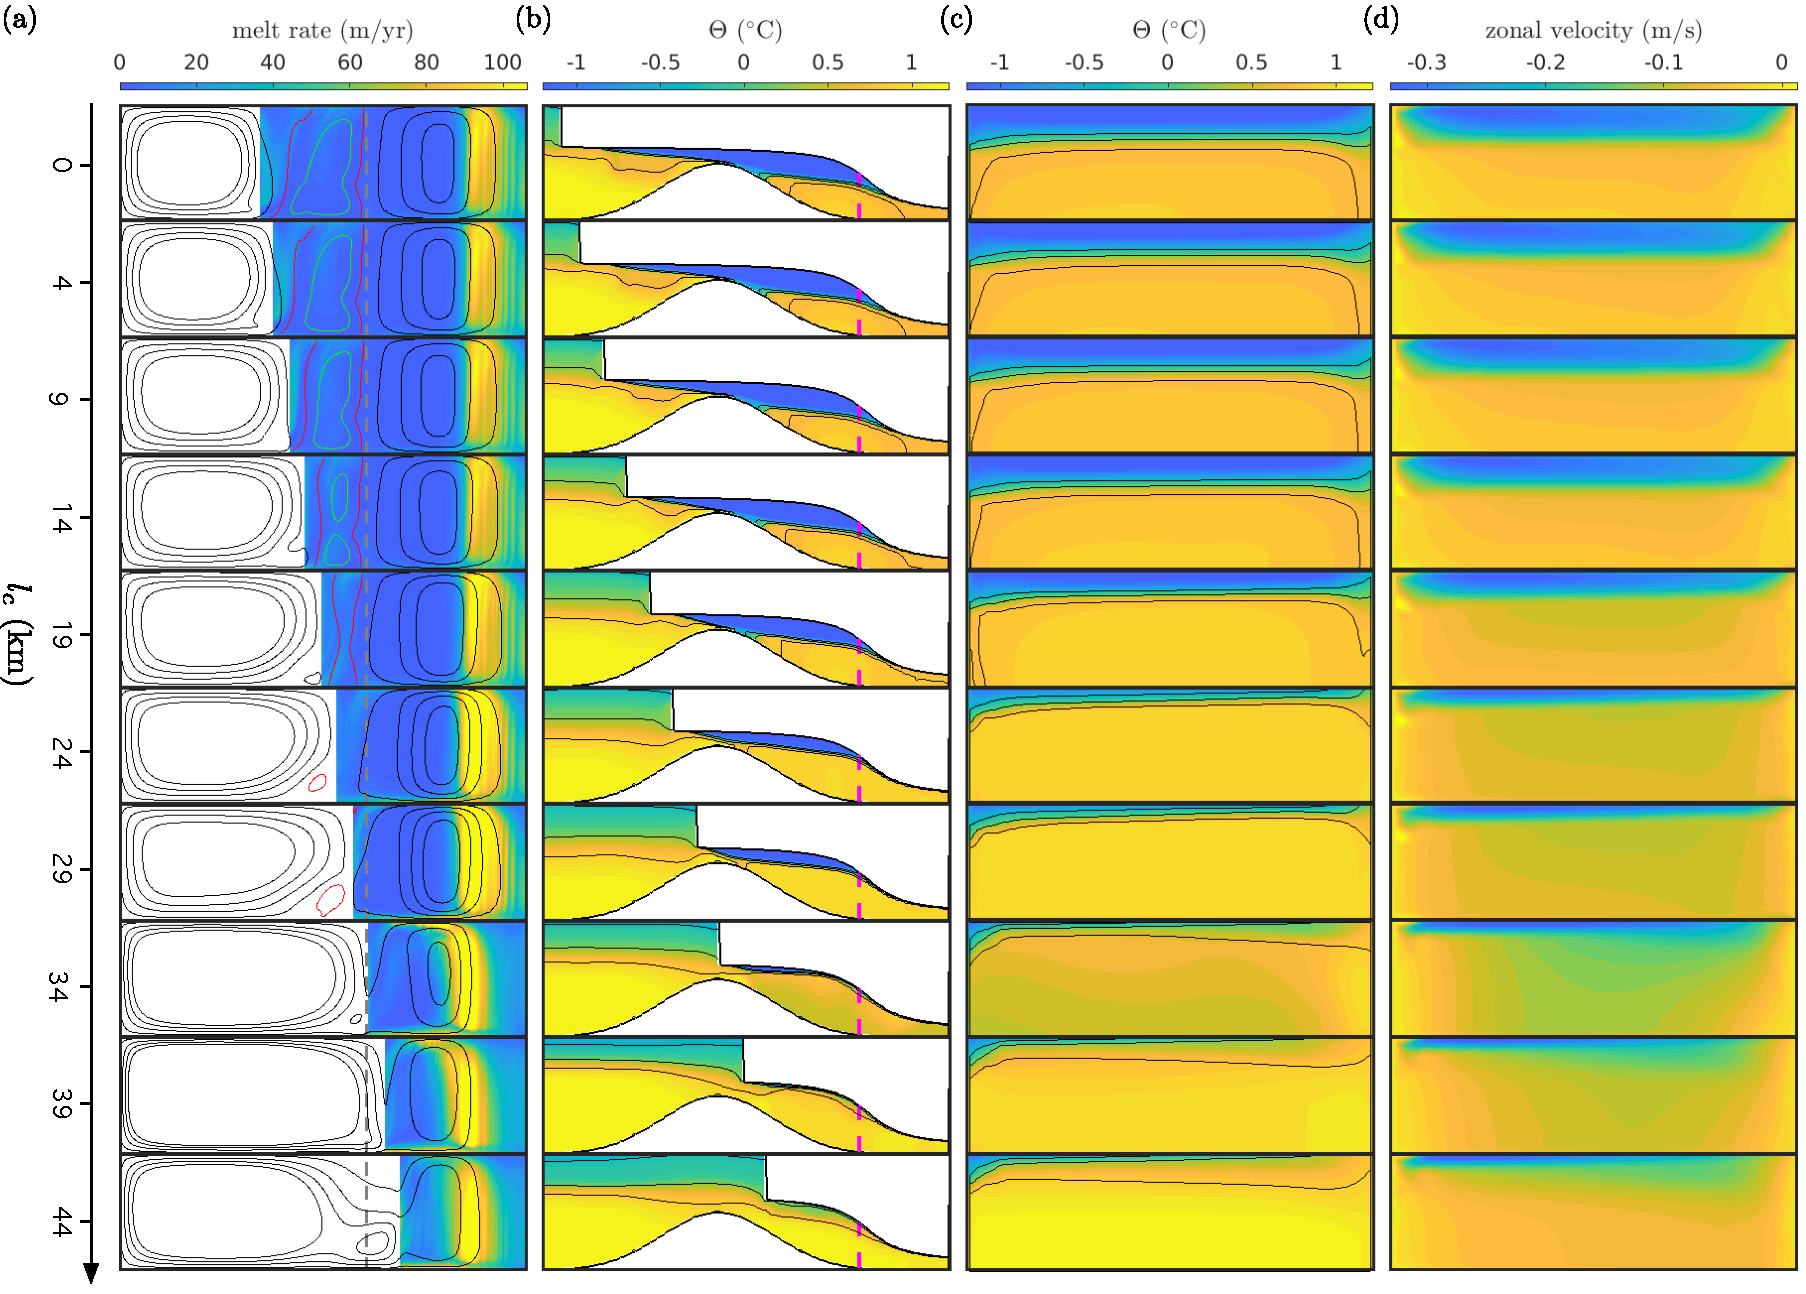
\includegraphics[width = 0.99\textwidth]{../make_figures/plots/figure5.pdf}
    \caption{(a) Contour plots of melt rate (colors) and barotropic stream function (contours, black at -0.1, -0.3, -0.5, and -0.7~Sv levels, magenta at the 0~Sv level, and green at the 0.05~Sv level) in the idealized simulations with $P = 600$~m and $W$ = 100~m. The calved length $l_c$ increases from 0~km in the first row to 44~km in the final row. The white sections indicate open ocean. (b) Contour plots of potential temperature $\Theta$ (colors) and salinity (contours, at levels 34.2, 34.4, and 34.6~PSU, i.e. as in figure~\ref{fig:figure3}) taken along the centreline of the domain (magenta dashed line in figure~\ref{fig:figure3}a). The white section at the top and bottom of each subplot indicate the ice shelf and seabed ridge, respectively. (c) Contour plots of potential temperature (colors) and salinity (contours, at levels 34.2, 34.4, and 34.6~PSU) along a zonal section located 20~km downstream of the grounding line [magenta dashed line in (b)]. (d) As in (c) with colors indicating the zonal velocity.  In each case, the color bar at the top of the column is appropriate for each row in the column. }
    \label{fig:figure5}
\end{figure}

%how can we understand what happens.
As mentioned, we shall assess the impact of calving on the behaviour primarily by considering its effect on the barotropic dynamics. To that end, we consider also the `barotropic velocity effect', $U_{be}(\ell_c)$, which is computed as in~\eqref{E:MillgateDecompU} albeit with barotropic, rather than boundary layer, velocities:
\begin{linenomath*}
\begin{equation}\label{E:MillgateDecompUbaro}
    U_{be}(l_c)  =  \frac{\int_{\text{IC}}~|\hat{\mathbf{u}}(x,y; l_c)|~\Delta T(x,y;l_c = 0)~\mathrm{d}x\mathrm{d}y}{\int_{\text{IC}}~|\hat{\mathbf{u}}(x,y; l_c = 0)|~\Delta T(x,y;l_c = 0)~\mathrm{d}x\mathrm{d}y},
\end{equation}
\end{linenomath*}

The agreement between $U_e(\ell_c)$ and $U_{be}(\ell_c)$ (figure~\ref{fig:figure4}b) suggests that changes in boundary layer velocity are closely related to changes in barotropic velocity, and provides support for our use of barotropic framework when diagnosing the melt response to calving.  %i.e. changes to the boundary layer velocity that result from changes in baroclinic flow that result from stratification are not important}


%Before proceeding, it is instructive to return to the barotropic equation~\eqref{E:BPVeq}. Given that the water column depth is uniform in $x$, the steady form of equation~\eqref{E:BPVeq} reduced to:
%\begin{equation}\label{E:BPVeq_reduced}
%    v f  \frac{\mathrm{d}}{\mathrm{d}y} \left(\frac{1}{h}\right) + \mathbf{u}.\nabla %\left(\frac{\zeta}{h}\right) = \text{viscous stresses.}
%\end{equation}
%\blue{Equation~\eqref{E:BPVeq_reduced} informs us that whenever there is meridional flow, it creates a planetary BPV source which must be balanced by either relative vorticity or viscous stresses. Viscosity requires high speeds to generate vorticity through shear. Therefore, which of relative vorticity or viscosity balances planetary BPV depends on the size of the gradient in the water column thickness: on the one hand, if the ocean is presented with a large gradient in water column thickness [large $\mathrm{d}/\mathrm{d}y(1/h)$], the resulting large planetary BPV source is balanced by viscous sources, which require rapid flow to generate the required shear. On the other hand, if the ocean is presented with a small gradient in water column thickness [small $\mathrm{d}/\mathrm{d}y(1/h)$], the planetary BPV source is weak and can be balanced by a relative vorticity source, which is associated with smaller flow speeds. This latter will be manifested as curved barotropic streamlines. In other words, equation~\eqref{E:BPVeq_reduced} implies that rapid changes in water column thickness will require high speed flow for a balance, while more gentle can be balanced by low speed flow but curved streamlines. In the baseline simulation described in the previous section, the gradient in water column thickness inshore of the ridge is large, and thus the circulation is vigorous. In this region, we see streamlines predominantly follow contour of constant water column thickness (figure~\ref{fig:figure4}c, d), confirming that relative vorticity in unimportant, and viscous sources of viscosity are primarily balancing planetary BPV. However, the gradient in water column thickness offshore of the ridge is weaker and can thus be balanced by variations in relative vorticity (note the curved streamlines in the outer cavity in figure~\ref{fig:figure4}c, d). }

%\red{Note that both relative vorticity (second on the left-hand side) and viscous terms (right-hand side) in~\eqref{E:BPVeq_reduced} scale with the flow speed. A faster flow will therefore tend to increase these terms, hence they will be able to match a stretching BPV requirement (first term on the left-hand side) more easily. Thus, regions in the vicinity of a stronger topographic barrier [higher $\partial / \partial x (1/h)$], be associated with a strong barotropic flow.}

We diagnose the melt response to calving by considering two regimes. In the first regime, the ice front is located offshore of the ridge, $\ell_c < 30$~km and much of the behavior is qualitatively similar to the uncalved case. The strong BPV barrier provided by the ridge and ice draft remains in place, and barotropic flow is unable to cross the ridge. The modest transport of warm water across the ridge, towards the inner cavity, occurs primarily via a baroclinic current at the eastern boundary, and the cavity circulation is vigorous. A topographically constrained cyclonic circulation is spun up inshore of the ridge, and this remains disconnected from the cyclonic circulation in the open ocean (figure~\ref{fig:figure5}a). There is little circulation in the outer cavity, which sits between these two cyclonic circulations. 

As ice front retreat proceeds within this regime, the total meltwater flux reduces ($\ell_c = 0-29$~km in figure~\ref{fig:figure5}b--c). This reduction is the non-trivial outcome of a competition between a reduction in melting area and an increase in ocean temperature inshore of the ridge as the ice shelf front is retreated. On the one hand, a smaller ice shelf means a reduction in the area over which melting is applied, promoting a reduced meltwater volume. On the other hand, a reduction in meltwater leads to reduced mixing between the cold outflow and the warm inflow across the ridge, so the temperature of the warm water that enters the cavity increases, promoting an increased melt rate.  We see that the effect of reductions in shelf area slightly outweighs the associated increase in melt rate when determining the overall meltwater flux. This is consistent with an increase in the thermal driving for $\ell_c < 30$~km  (figure~\ref{fig:figure4}b). The associated increase in melt rate in the inner cavity leads to a stronger buoyancy flux, driving a slightly stronger circulation (increase in $U_{be}$ in figure~\ref{fig:figure4}b), which itself enhances melting locally.


%what happens when ice front approaches the ridge? barotropic flow may cross the ridge because ice front is a leaky PV barrier. This flow floods inner cavity with warm water. However, the discontinuity in 1/h is now significantly reduced in the inner cavity, leading to a reduction in the strength of the circulation.
The second regime takes effect when the ice front is located above the seabed ridge crest. In this case, only a single PV barrier -- the ice front, which sits at the ridge crest -- remains. The region offshore of the ridge, which previously hosted a weak circulation that separated the strong cyclonic gyres in the open ocean and in the region inshore of the ridge, no longer exists, permitting these two gyres to connect dynamically. The flow at the ridge crest now has a vigorous barotropic component. North-south barotropic flow across the ridge is therefore permitted because the planetary vorticity requirement associated with such flow can be satisfied by viscous sources associated with the ice front. Thus, a barotropic flow of approximately 0.1~Sv is able to cross the ridge at its eastern side (figure~\ref{fig:figure5}a), providing a large amount of heat to the inner cavity, while meltwater is efficiently flushed out of the cavity on the western side of the ridge. The region inshore of the ridge is almost entirely flooded with warm water (figure~\ref{fig:figure5}c). Although this means that there is much more heat available for melting (thermal driving effect increases when the ice front coincides with the ridge crest, figure~\ref{fig:figure4}b), the more efficient cavity flushing leads to a concomitant reduction in circulation (figure~\ref{fig:figure5}d). The latter outweighs the increase in thermal driving, ultimately leading to a reduction in the melt rate (figure~\ref{fig:figure4}b).

%Again, viscosity at the ice front permits barotropic flow to break the topographic constraint at this BPV barrier, but, since this barrier is now at the ridge crest, the result is that a significant barotropic flow (approximately 0.1~Sv) is permitted to cross the ridge (figure~\ref{fig:figure5}a). This flow is far more effective at flushing the inner cavity than the boundary current that flushes it when the ice front is located further offshore; as a result, the inner cavity is almost entirely flooded with warm water (figure~\ref{fig:figure5}c), which means that there is much more heat available for melting (thermal driving effect increases when the ice front coincides with the ridge crest, figure~\ref{fig:figure4}b). However, the concomitant reduction in circulation outweighs the increase in thermal driving, leading to a reduction in the melt rate (figure~\ref{fig:figure4}b). \blue{This reduction in circulation can be rationalized by returning to equation~\eqref{E:BPVeq_reduced}: the gradient in water column thickness has been relaxed so that planetary BPV sources can be balanced by relative vorticity, rather than viscosity and a much slower the flow can support a balance with planetary vorticity sources. (The curved streamlines inshore of the ridge for $\ell_c = 34$~km in figure~\ref{fig:figure5}b indicate that relative vorticity is now playing a more important role.)}

This picture remains when the ice front is retreated beyond the ridge. The gyres in the open ocean in the region inshore of the ridge are connected, permitting a significant barotropic flow to cross the ridge, which efficiently flushes the inner cavity with warm water. Thermal driving is enhanced, but cavity circulation is reduced, when compared to the situation in which the ice front is located offshore of the ridge. Melt rates become independent of ice front position once the ice front has retreated beyond the ridge. This indicates that the ridge only plays a role in the melt response to calving when it has an ice shelf overlying it (and the ridge-draft gap is small enough, as will be shown).

In summary, when the ice front is located offshore of the ridge, the ridge-draft BPV barrier prevents barotropic flow into the cavity and the inner cavity is weakly flushed with warm water via a baroclinic boundary flow at the eastern wall. As the ice front retreats, mixing with meltwater at this boundary is reduced; the heat content, and thus melt rate, in the inner cavity increases, leading to enhanced circulation and further increasing melt. As the ice front is retreated to the ridge crest, viscous vorticity exchanges at the ice front permit barotropic flow to cross the ridge. This flow efficiently flushes the inner cavity with warm water, providing a large amount of heat for melting, but is accompanied by a reduction in cavity circulation, which outweighs the increase in heat to ultimately reduce the inner cavity melt rate, compared to when the ice front is located offshore.


\section{Effect of Cavity Geometry on Melt Response to Calving}\label{S:Results:H}
%what are we doing here and why (briefly)
In the previous section, we analyzed how the inner cavity melt rate responds to ice front retreat, and discussed the mechanisms responsible, in the case that the gap between the ice draft and ridge-crest is narrow. The strength of the topographic barrier that restricts warm water access to the inner cavity was identified as an important control on this response. In this section, we describe how this picture changes for larger values of $W$ (in particular, for $W=150$~m and $W=200$~m), which lead to a weaker topographic barrier at the ridge crest.

%how do melt rates change
%In figure~\ref{fig:figure6}, we plot the inner cavity melt rate and velocity-thermal driving decomposition as a function of the calved length $l_c$ are plotted in figure for both $W$ = 150~m and $W$ = 200~m. Comparison with the corresponding results for $W$=100~m (figure~\ref{fig:figure6}a) indicates that at larger values of $H$, the inner cavity melt rate is less sensitive to calving: the range of inner cavity melt rates reduces from approximately 27\mpryr for $W$=100~m to 10\mpryr and 7\mpryr for $H$=150~m and $H$=200~m, respectively. In addition, the peak inner cavity melt rate is reached when the ice extent is greater ($l_c$ is smaller) as the gap $W$ is reduced (approximately 29~km, 14~km, and 10~km for $W$=100~m, 150~m, and 200~m, respectively).


\begin{figure}
    \centering
    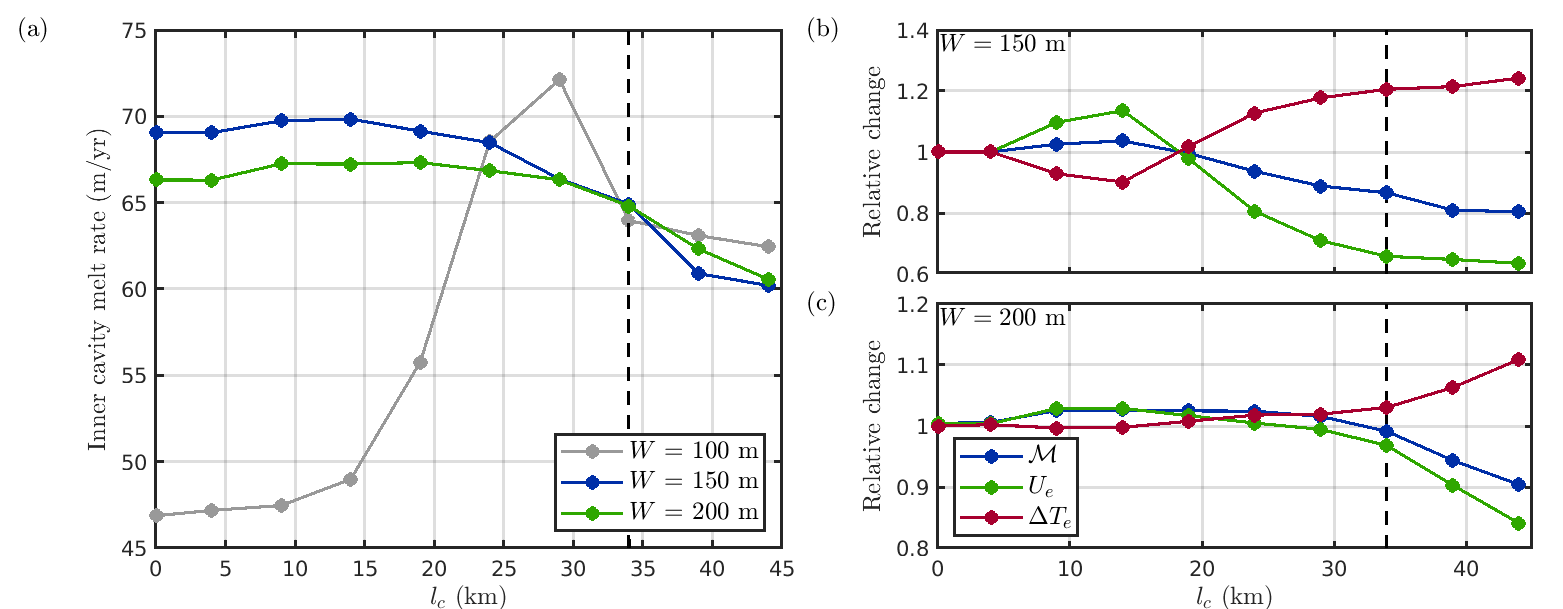
\includegraphics[width =
    \textwidth]{../make_figures/plots/figure6.png}
    \caption{(a) Inner cavity melt rate as a function of the calved length $l_c$ for $W=100$~m (grey, as in figure~\ref{fig:figure4}a), $W=150$~m (blue), and $W=200$~m (green), each with $P = 600$~m.  (b)--(c) Velocity-thermal driving decomposition for (b) $W = 150$~m and (c) $W = 200$~m. In each plot, the black dashed line indicates the position of the ice front when it is located directly above the seabed ridge.}
    \label{fig:figure6}
\end{figure}

\begin{figure}
    \centering
    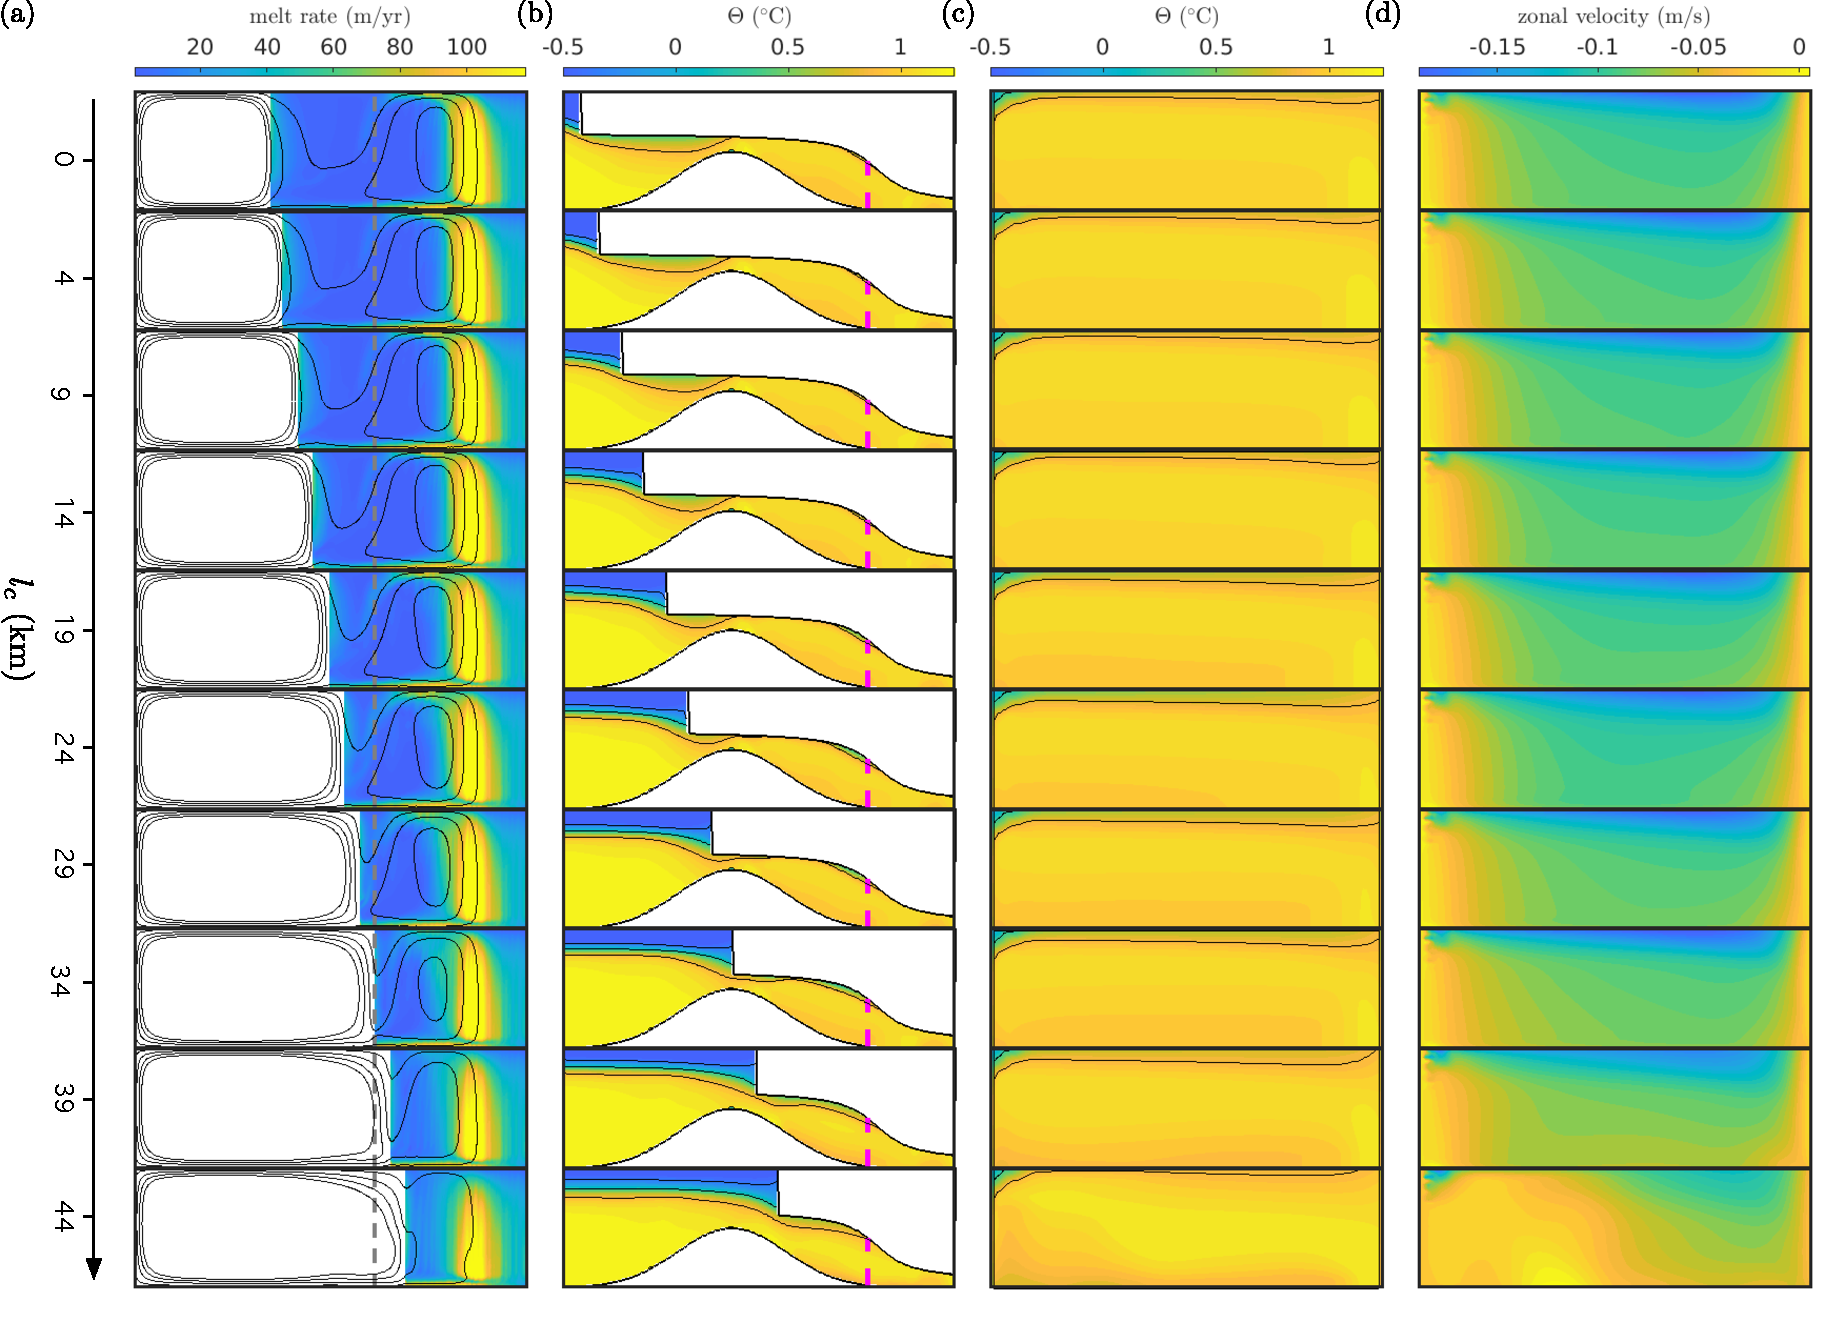
\includegraphics[width = \textwidth]{../make_figures/plots/figure7.pdf}
    \caption{Response of ocean characteristics to calving in the idealized experiments with $P=600$~m and $W=200$~m. This plot is as in figure~\ref{fig:figure5} for the experiment with $W=200$~m.}
    \label{fig:figure7}
\end{figure}


%what do we see
Figure~\ref{fig:figure6}a shows the inner cavity melt rate as a function of calved length $l_c$ for $W=150$~m and $W=200$~m in the $P = 600$~m case. We focus first on the $W = 200$~m case, which is characterized by inner cavity melt rates that are largely independent of the ice front position. As before, we use a barotropic framework to diagnose the behavior; barotropic contours are shown, alongside zonal and meridional cross-sections, for this case in  figure~\ref{fig:figure7} (the corresponding figure for $W = 100$~m is figure~\ref{fig:figure5}). Recall that, in the $W=100$~m case, two regimes are observed, which are delineated by whether barotropic flow is able to cross the ridge or not: firstly, when the ice front is located offshore of the ridge, there is a `blocked' regime: the strong BPV barrier that the ridge-crest and ice draft presents means that barotropic flow is prevented from crossing the ridge and, secondly, there is a `connected' regime: when the ice front is located above, or inshore, of the ridge, the gyres in the open ocean and inshore of the ridge become dynamically connected and barotropic flow is able to cross the ridge. In the $W=200$~m case, however, the ridge-draft BPV barrier is much weaker than in the $W=100$~m case, and barotropic flow is able to cross the ridge, even when the ice front is located offshore of the ridge (figure~\ref{fig:figure7}a). The blocked regime is never realized: for all values of $\ell_c$, the regions inshore and offshore of the ridge are dynamically connected. The system always behaves in a qualitatively similar way to the $W = 100$~m connected regime, with the inner cavity efficiently flushed with modified CDW (figure~\ref{fig:figure7}b, c), and experiencing weak circulation. Ice front retreat therefore has little effect in the $W = 200$~m case. In particular, this removes the tendency for both increasing temperature and circulation that we see in the $W=100$~m case as the ice front is retreated towards the ridge. This invariance to ice front position also holds for larger ridge-draft gaps ($W>200$~m), a finding that is consistent with the results of~\citeA{DeRydt2014JGeophysResOceans}.

The $W = 150$~m case sits between the strong response to calving for $W = 100$~m, and the weak response to calving for $W = 200$~m. There are several similarities with the $W = 100$~m case: there is a reasonable sensitivity to ice front position (although it is somewhat smaller than in the $W = 100$~m case), the inner cavity melt rate reaches a maximum when the ice front is located offshore of the ridge crest, and the reduction in inner cavity melt rate for values of $\ell_c$ above that at which the maximum melt rate is attained results from a reduction in the inner cavity circulation that outweighs an increase in thermal driving (figure~\ref{fig:figure6}b). In contrast to the $W = 100$~m case, however, this scenario does not display a threshold-like behavior, where the inner cavity melt rate drops suddenly as the calving front reaches the top of the ridge. The weaker BPV barrier in the $W=150$~m case means that, as in the $W = 200$~m case, the blocked regime is never realized; the threshold behavior, which occurs at the transition between the two regimes, is therefore suppressed.


\section{Effect of Hydrographic Conditions on Melt Response to Calving}\label{S:Results:P}
Before moving on to assess how the inner cavity melt rate responds to calving in the realistic simulations, we briefly consider how the picture presented in the previous two sections changes depending on the choice of hydrographic forcing. Since we consider a constant ridge height, variations in the difference between the pycnocline depth and the depth of the ridge crest, which we expect to be a key driver of the quantity of warm water that is able to spill over the ridge and into the inner cavity, is captured here by variability in the value of $P$ (figure~\ref{fig:figure2}).

\begin{figure}
    \centering
    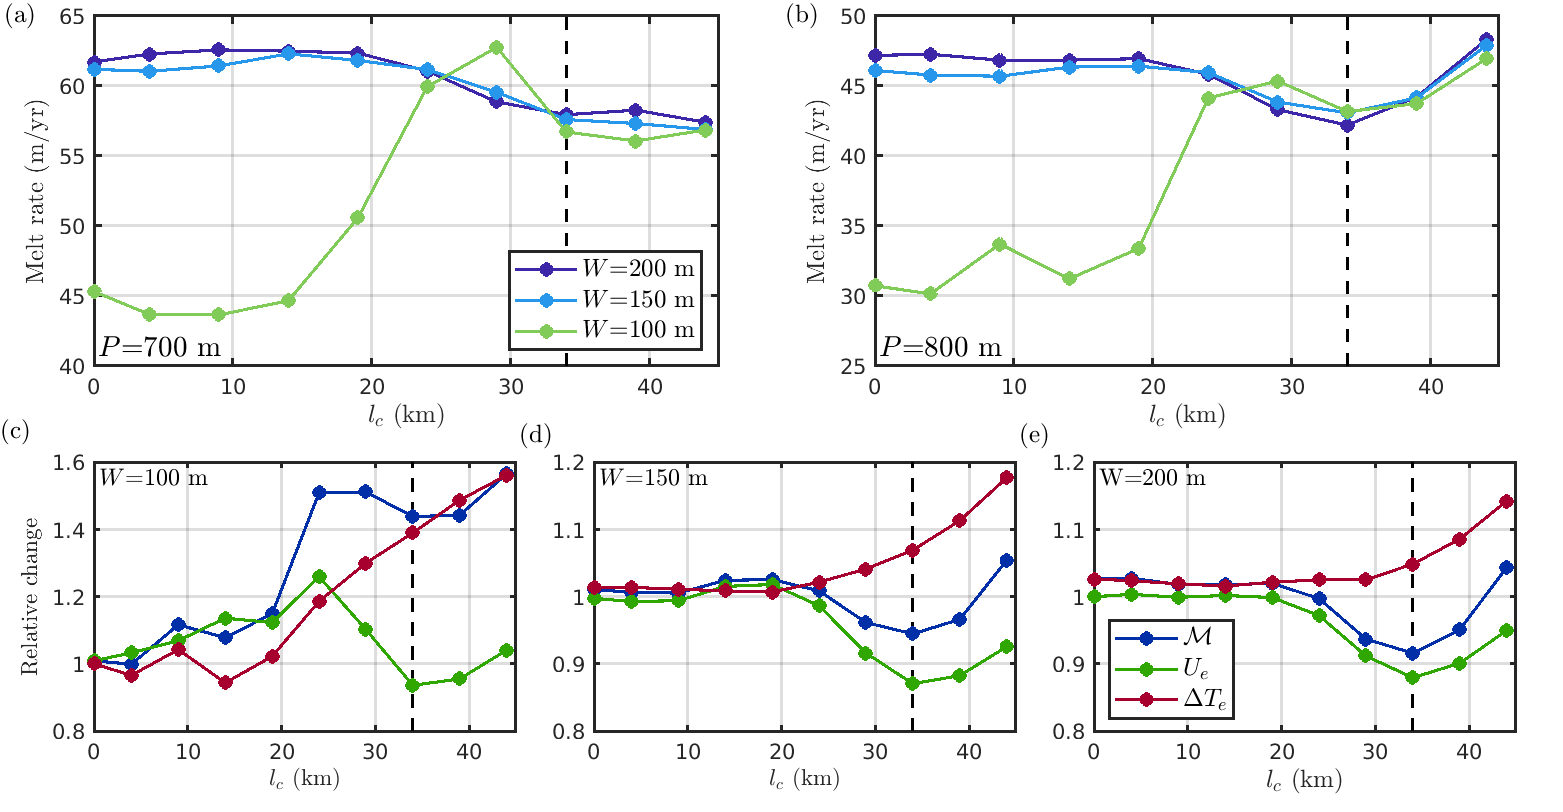
\includegraphics[width = \textwidth]{../make_figures/plots/figure8.png}
    \caption{(a)--(b) Inner cavity melt rate as a function of calved length $l_c$ in idealized simulations with (a) $P$=700~m and (b) $P$=800~m. Colors correspond to different values of $W$, as indicated by the legend in (b). The black dashed line indicates the location of the crest of the seabed ridge. The inset in (a) shows the sensitivity to the pycnocline position -- the ratio of the inner cavity melt rate for $P = 700$~m and $P = 800$~m [i.e. the ratio of the data represented by the green lines in (a) and (b))] -- as a function of the calved length $l_c$. (c)--(e) Velocity--thermal driving decompositions (as in figure~\ref{fig:figure4}) for the $P = 800$~m data shown in (b): (c), (d), and (e) correspond to the results for $W=100$~m, $W=150$~m, and $W=200$~m, respectively, as indicated.}
    \label{fig:figure8}
\end{figure}


% Introduce simulations with reminder of what they correspond to
The inner cavity melt rate and velocity-thermal driving decomposition for the experiments with $P=700$~m (hydrographic forcing as in the dashed profiles in figures~\ref{fig:figure2}b and c) and with $P=800$~m (dot-dashed profiles) are shown in figure~\ref{fig:figure8}a and b, respectively. The results for $P=700$~m are similar to those for $P=600$~m: for the narrowest gap ($W=100$~m), the inner cavity melt rate is sensitive to the ice front position, increasing rapidly as the ice front is retreated towards the ridge crest, before dropping off sharply when the ice front reaches it, and does not change under further ice front retreat beyond the ridge. In addition, the sensitivity of melt rate response to calving reduces as the gap widens. A velocity-thermal driving decomposition for the experiments with $P=700$~m (not shown) is qualitatively similar to the $P=600$~m case discussed above, suggesting that the mechanisms for the response are as discussed in \S\ref{S:Results:lc}. The similarity between the $P=600$~m and $P=700$~m cases is perhaps unsurprising when framed in terms of the relationship between the depth of the pycnocline and the height of the ridge crest: in both cases, the CDW layer extends all the way to the top of the ridge (see figure~\ref{fig:figure2}) and thus the seabed ridge alone does not provide a significant barrier to CDW access to the inner cavity.

%results are different for P = 800 -- how?
In the $P=800$~m case, while the ice front is located offshore of the ridge, the melt rate is either constant, or increases, as the ice front is retreated, depending on the value of $W$ (figure~\ref{fig:figure8}b). A reduction in the ice-ocean boundary layer velocity is responsible for a slight drop in inner cavity melt rates as the ice front is retreated towards the ridge crest (figure~\ref{fig:figure8}c--e), as in the $P=700$~m and $P=600$~m cases. Beyond this point, the $P=800$~m case differs from the $P = 600$~m and $P = 700$~m cases: retreating the ice front beyond the ridge results in an increase in the inner cavity melt rate (figure~\ref{fig:figure8}b), which is associated with a reversal of the reduction in boundary layer velocity (figure~\ref{fig:figure8}c--e) (i.e. the boundary layer velocity increases on average when the ice front is retreated beyond the ridge). The important difference in this case is that the seabed ridge alone is able to provide a significant barrier that prevents warm water from reaching the inner cavity (the CDW layer in the outer cavity does not extend over the top of the ridge, see figure~\ref{fig:figure9}). As calving proceeds beyond the ridge, the thermal driving does not saturate (as in all the cases discussed above), but continues to increase, and the concomitant increase in glacial melt results in a stronger circulation (figure~\ref{fig:figure8}c).

\begin{figure}
    \centering
    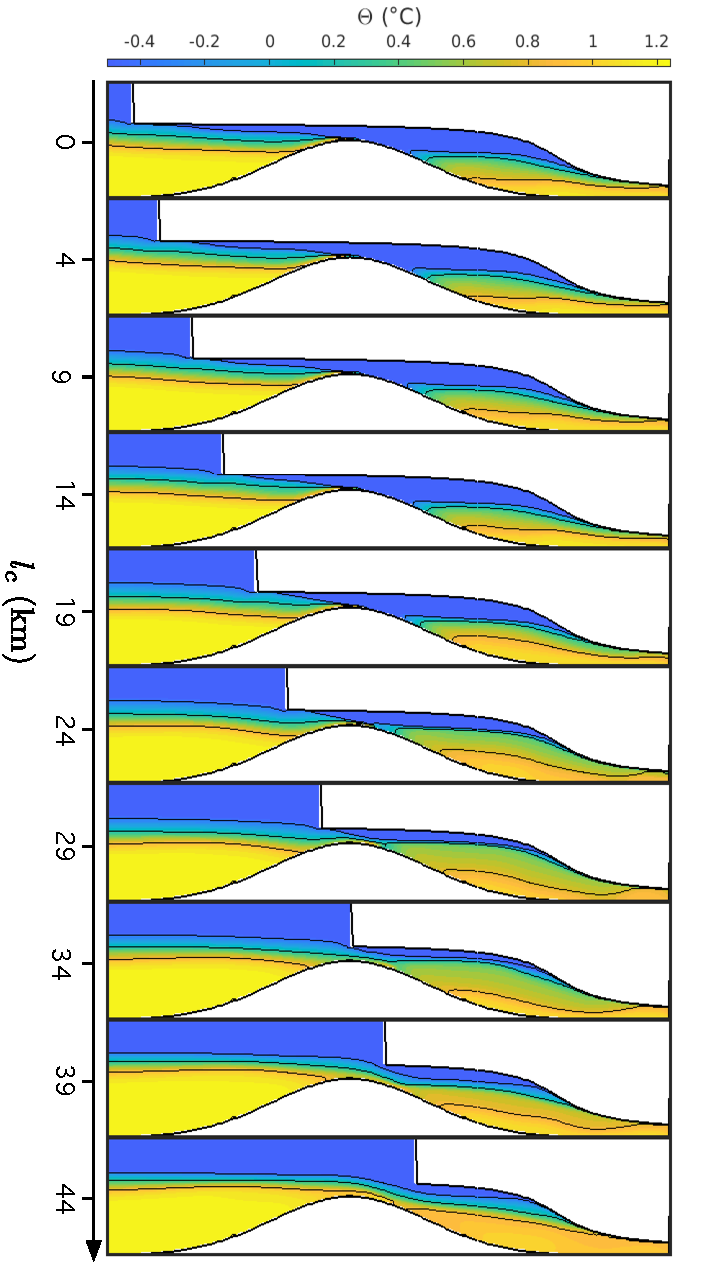
\includegraphics[width = 0.35\textwidth]{../make_figures/plots/figure9.pdf}
    \caption{Meridional cross-sections, as in figure~\ref{fig:figure5}b for the simulation with $P=800$~m, $W=100$~m. }
    \label{fig:figure9}
\end{figure}

\section{Assessing the Melting Response of PIIS to Calving}\label{S:Realistic}
% intro to the section
The experiments described in \S\ref{S:Experiment}--\ref{S:Results:P} reveal how melt rates near the grounding line in idealized geometries with a uniform ridge-draft gap may respond sensitively to calving, depending on the thickness of the ridge-draft gap. These idealized experiments inform our understanding of similar experiments in a realistic domain, which are designed to assess the response of melt rates to PIIS calving. In this section, we describe these experiments, and present and analyze the results.

\begin{figure}
    \centering
    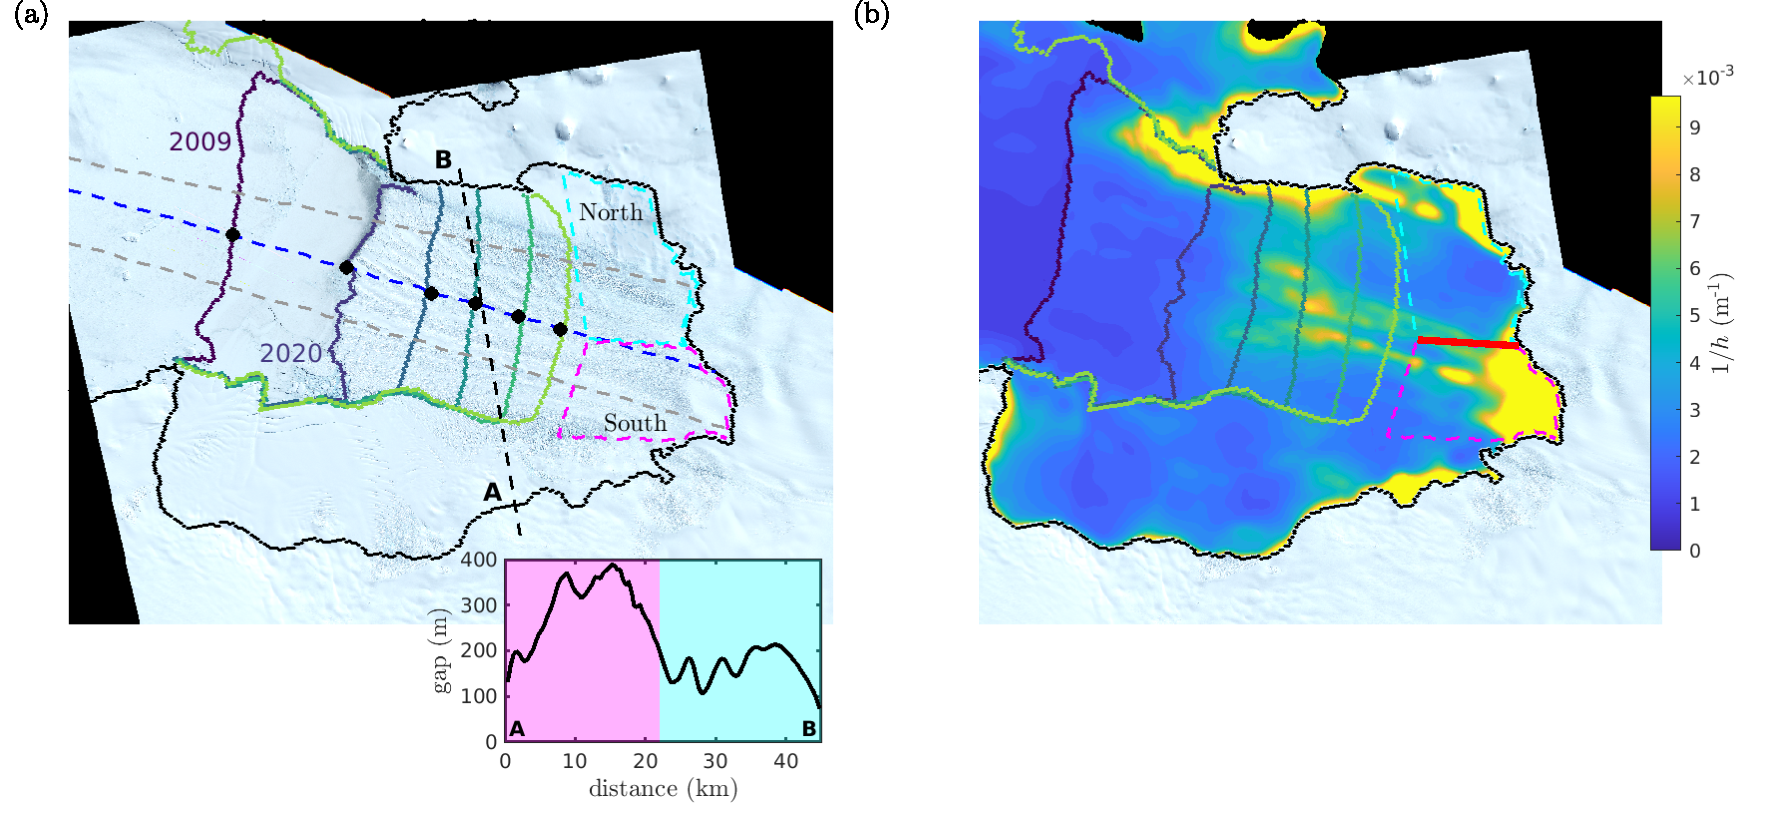
\includegraphics[width =\textwidth]{../make_figures/plots/figure10.pdf}
    \caption{(a) Ice front positions used in experiments designed to assess the response of the PIIS melt rate to calving. Each experiment considers to a different ice front position, indicated by the curves in the purple to green colormap; labelled dark purple and dark blue ice fronts correspond to the 2009 and 2020 front positions, respectively. The solid black line indicates the location of the 2009 grounding line from~\citeA{Joughin2010GRL}. The blue dashed line roughly indicates the centreline of the cavity, along which the calved length -- the difference between the ice front in the respective experiments and the 2009 ice front -- is measured, and the black dashed line approximately indicates the peak of the seabed ridge. The cyan (north) and magenta (south) boxes indicate the inner cavity regions considered in the experiments (see main text). Inset: plot of the (vertical) gap between the ridge crest and the ice draft, measured along the black dashed line in the main figure. Cyan and magenta shaded sections correspond to locations north and south of the blue dashed centreline, respectively. The background image is a Sentinel 2 mosaic from November 2020. (b) Inverse water column thicknesses $1/h$ used in the experiment with the 2009 ice front. Ice front positions, inner cavity regions, and black dashed ridge crest are as in (a).  Note that the boundary between the inner cavity regions (solid red line) is approximately aligned with a region of locally enhanced $1/h$, indicating the presence of a barotropic potential vorticity barrier between the north and south inner cavity regions.}
    \label{fig:figure10}
\end{figure}

%Describe experiments
\subsection{Experiment Details}
Our experiments with a realistic setup are designed to assess the possible response of PIIS melt rates to calving in practice. To do so, we solve for the three-dimensional, quasi-steady ocean circulation and associated melt rates simultaneously in a PIG cavity geometry [from~\citeA{Dutrieux2014Science}, and described briefly below], using the ocean model described in \S\ref{S:Experiment:Model}. We consider six different ice shelf topographies, each of which has a unique ice front position. The locations of these ice fronts are shown in figure~\ref{fig:figure10}: the first experiment (`2009' labelled curve in figure~\ref{fig:figure10}a) uses an ice shelf geometry that corresponds to PIIS in 2009~\cite{Dutrieux2014Science}. The second experiment (`2020' labelled curve in figure~\ref{fig:figure10}a) uses the 2009 ice shelf draft, but with a section of ice removed so that the ice front matches that obtained in 2020, who position is determined from a Sentinel 2 mosaic of PIG). The four further experiments similarly use the 2009 ice shelf draft but with sections of fast flowing ice (i.e. within the shear margins) removed (figure~\ref{fig:figure10}). We stress that, as in the idealized experiments, the ice thickness, and thus grounding line position and ice shelf draft, at existing shelf locations remains the same in each experiment, and only the ice front position varies.

%how do we get cavity and draft
The sub-ice shelf cavity geometry we use is computed from the ice and seabed geometry, as described by~\citeA{Dutrieux2014Science}. Briefly, the ice shelf geometry is calculated from a 40~m-resolution digital elevation model (DEM) of the ice freeboard from 2008~\cite{Korona2009Photogrammetry}, which is adjusted with a constant median bias from observations obtained from the Autosub underwater autonomous vehicle~\cite{Jenkins2010NatureGeo}. The DEM assumes freely floating ice throughout the shelf, which may reduce its accuracy close to the grounding line. Over the continental shelf, the seabed geometry is well known from ship echo-sounding \cite{Dutrieux2014Science}, while in the cavity it is calculated from an inversion of gravimetry data and corrected point-wise using the median difference between the depth from the gravimetry inversion and the Autosub observations.

%model notes and calibration
We consider a single hydrographic forcing, corresponding to observed 2009 conditions in Pine Island Bay (dark grey lines in figure~\ref{fig:figure2}b--c), to which the ocean is restored far from the ice shelf. All model parameters, and the spin-up procedure, are as in the idealized experiments, as described in \S\ref{S:Experiment:Model}. In particular, we take the drag coefficient in the three-equation formulation of melting to be 4.5$\times10^{-3}$; this value is tuned so that the total meltwater flux in the simulation with the 2009 geometry (86~km\textsuperscript{3} year\textsuperscript{-1}) closely matches the estimated observed total meltwater flux for 2009 (80~km\textsuperscript{3} year\textsuperscript{-1}) \cite{Dutrieux2014Science}.

%gap is not uniform, but sort of split. Tell the reader what the different regions are.
As mentioned, the ridge-draft gap under PIIS is not uniform but varies from approximately 100~m at its narrowest to 400~m at its widest.  The ridge-draft gap (inset in figure~\ref{fig:figure10}) can be approximately partitioned into a northern section, where the gap is relatively thin, and a southern section, where the gap is relatively thick. A region of locally elevated $f/h$ running east-west (solid red line in figure~\ref{fig:figure10}b) meets the north-south aligned seabed ridge at the junction between these wide and narrow sections (see figure~\ref{fig:figure10}); this east-west aligned section is created by a thick ice keel in the center of the ice stream and extends all the way to the grounding line, partitioning the region inshore of the north-south aligned ridge into a northern inner cavity (cyan box in figure~\ref{fig:figure10}a) and a southern inner cavity (magenta box). The east-west aligned section of locally elevated $f/h$  provides a PV barrier between the two inner cavity regions, which are therefore approximately dynamically disconnected (figure~\ref{fig:figure11}a). In the following, we therefore evaluate the melt response to calving in the two inner cavity regions separately.

\begin{figure}
    \centering
    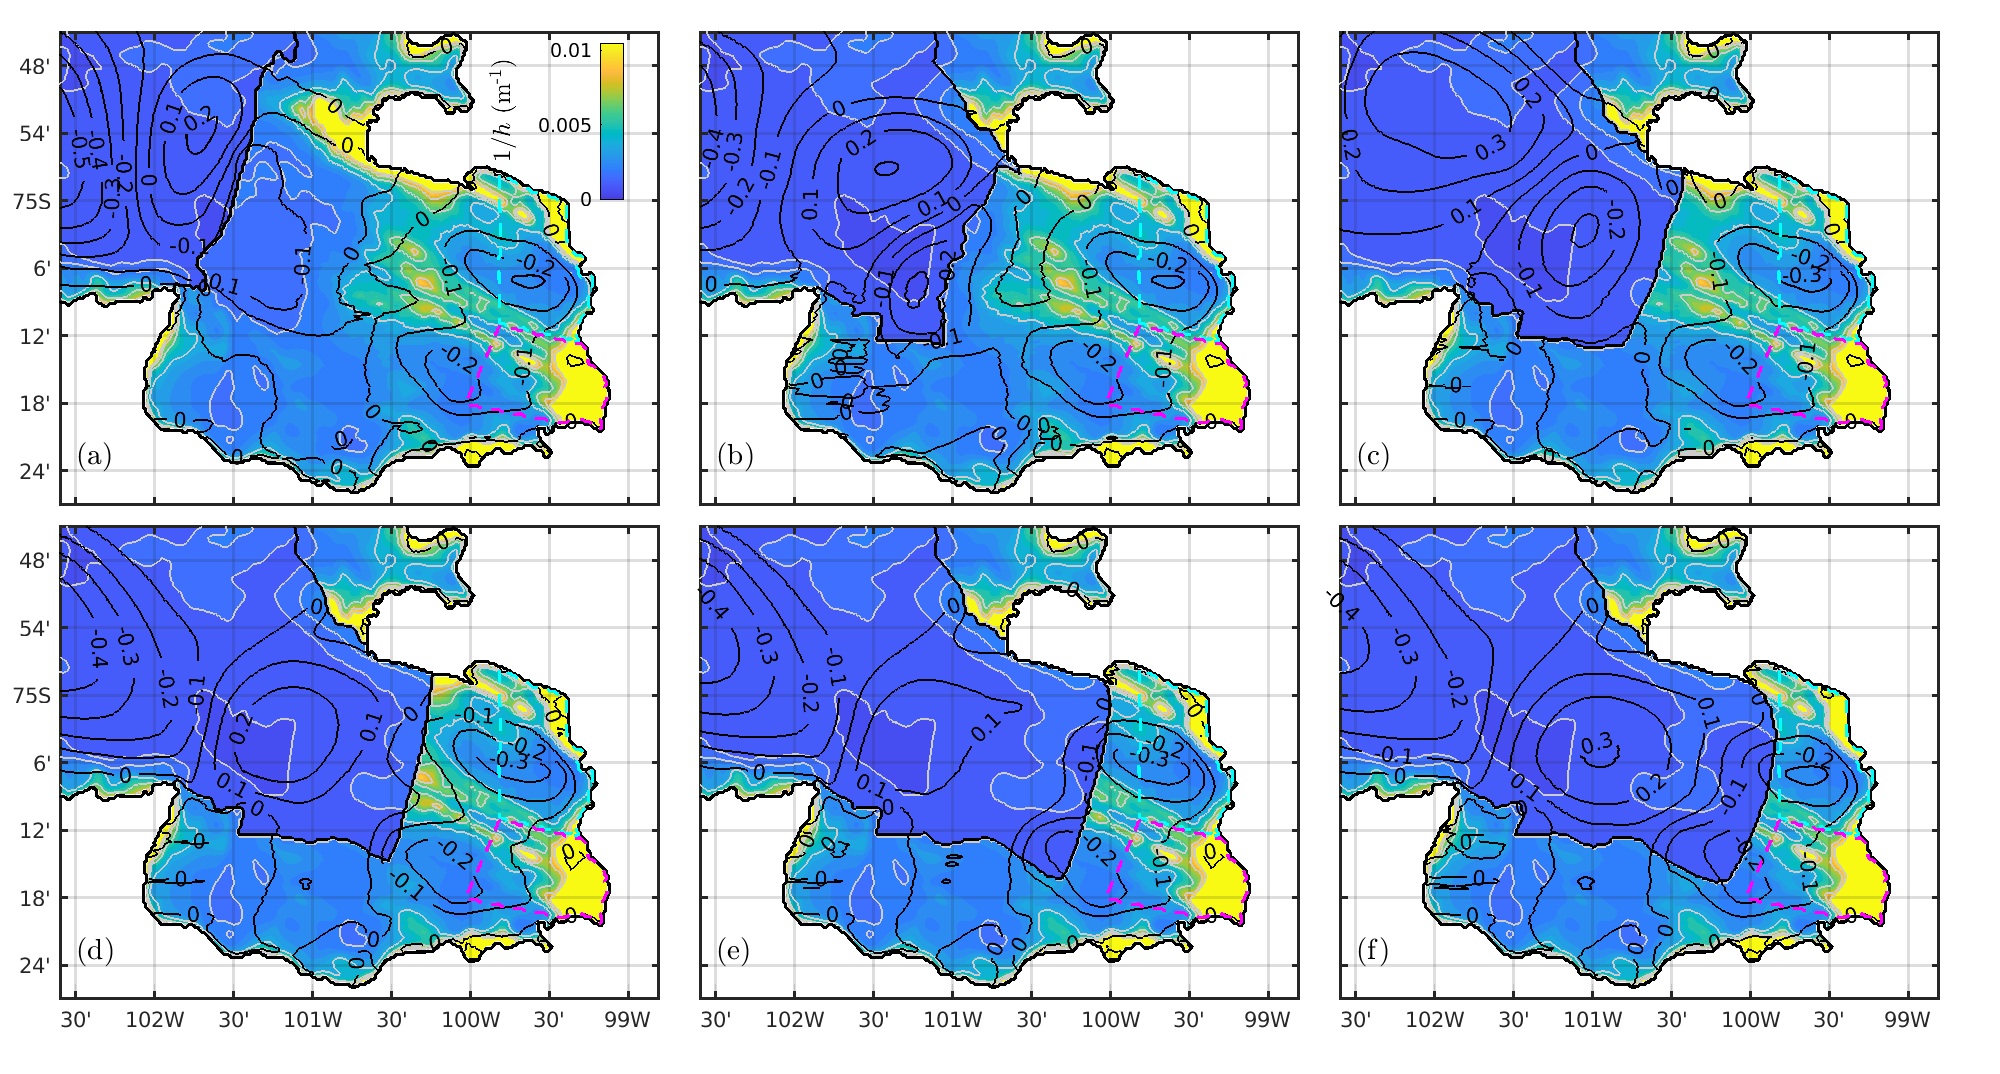
\includegraphics[width = \textwidth]{../make_figures/plots/figure11.png}
    \caption{Simulated barotropic stream function (labelled black contours) and inverse water column thickness $1/h$ (colors and gray contours at levels corresponding to 200, 400, 600, 800, and 1000~m water column thickness). Magenta and cyan dashed boxes indicate the extent of the north and south inner cavity regions, respectively.}
    \label{fig:figure11}
\end{figure}


\subsection{Results}

\begin{figure}
    \centering
    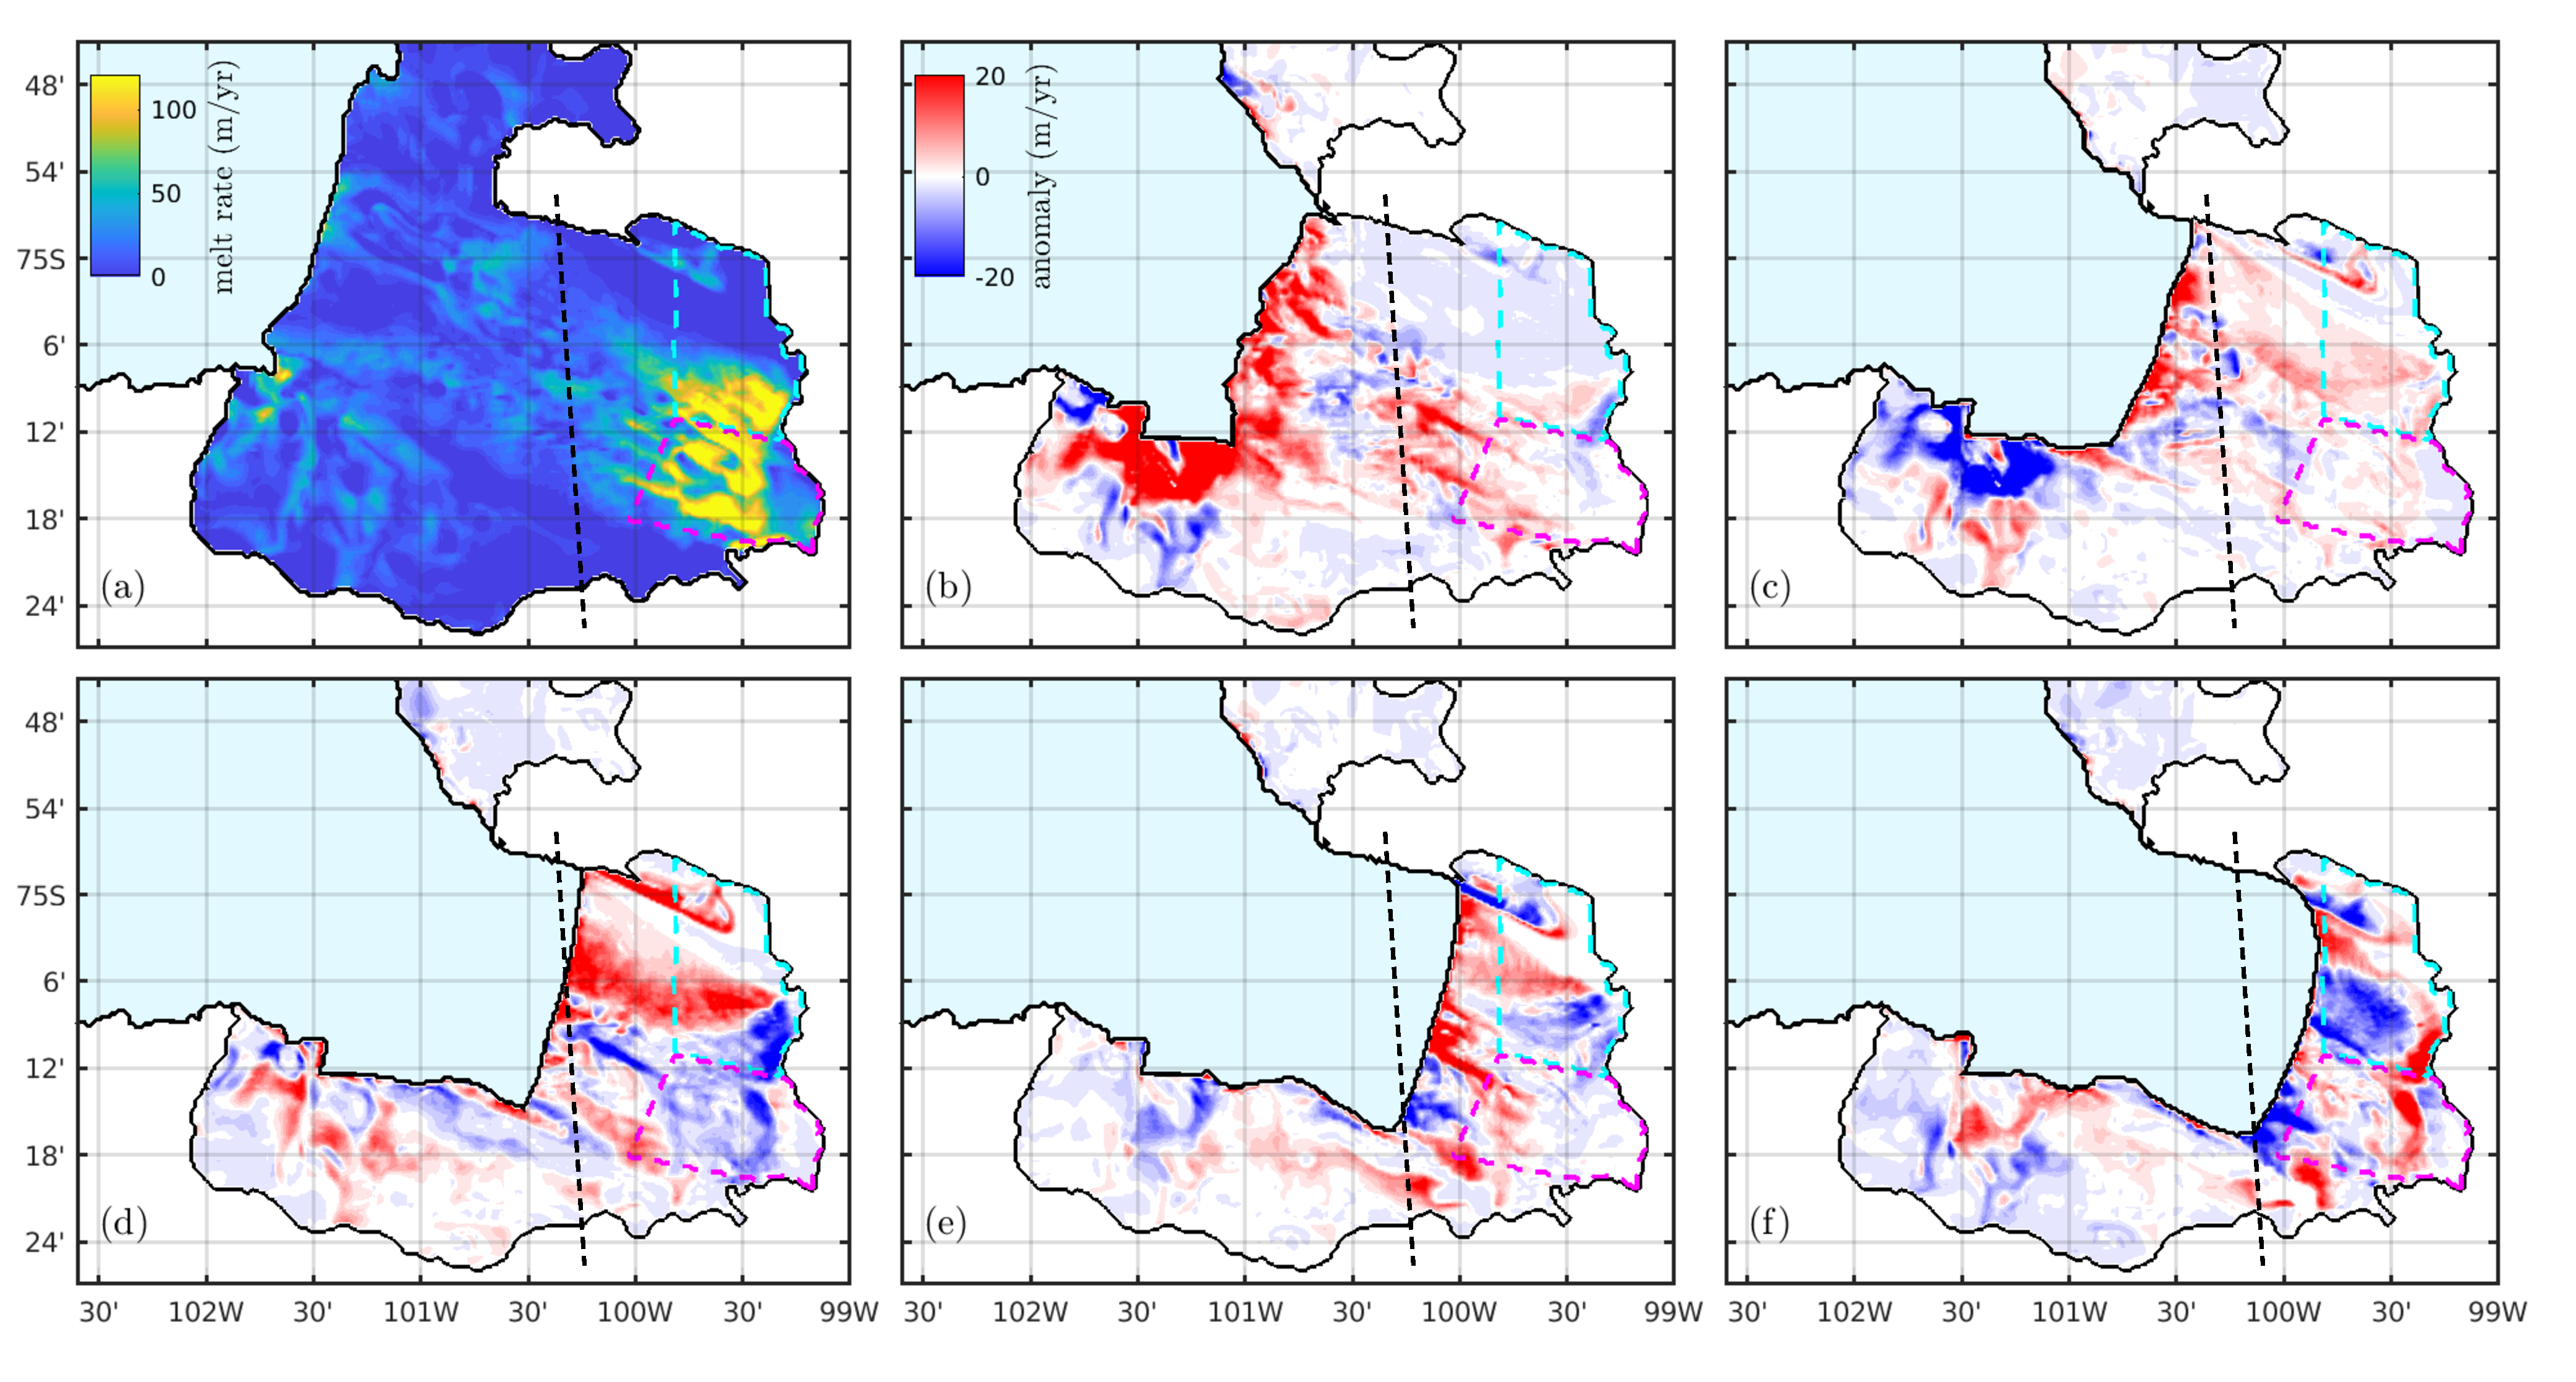
\includegraphics[width = \textwidth]{../make_figures/plots/figure12.pdf}
    \caption{(a) Simulated melt rate in the 2009 Pine Island geometry. Cyan and magenta dashed boxes [also in (b)--(f)] indicate the north and south inner cavity regions (see figure~\ref{fig:figure10}), where the highest melt rates are concentrated. (b)--(f) Non-cumulative melt rate anomaly in the simulations (i.e. measured relative to the previous panel). The colorbar in (b) is appropriate for each of (b)--(f). Note that melt rate anomalies in (b) are saturated to a maximum of 20~m~year\textsuperscript{-1} in the vicinity of the ice front (the maximum anomaly is approximately 30~m~year\textsuperscript{-1}). In each case, the ice shelf front and 2009 grounding line, which are from \citeA{Joughin2010GRL}), are shown as a solid black line, and an estimate of the location of the ridge crest is shown as a black dashed line.}
    \label{fig:figure12}
\end{figure}


%introduce simulations
Cavity circulation (figure~\ref{fig:figure11}a) and melt rates (figure~\ref{fig:figure12}a) in the uncalved (2009) experiment are qualitatively similar to the corresponding baseline idealized experiment: melt rates are concentrated near to the grounding line, reaching a peak of approximately 120~m year\textsuperscript{-1} several kilometers downstream of it, while remaining below 20~m~year\textsuperscript{-1} over the majority of the shelf. This pattern of simulated melt rates under PIIS is consistent with observations~\cite{Dutrieux2013Cryosphere} and other numerical simulations of cavity circulation under PIIS~\cite[for example]{Heimbach2012AnnGlac}. Cyclonic circulation spins are spun up within both inner cavity sections, and in the open ocean offshore of the ice front, while a weak anti-cyclonic circulation spins up in the outer cavity between the seabed ridge and the ice front. Barotropic stream function contours largely follow the contours of constant water column thickness (figure~\ref{fig:figure11}).

Figure~\ref{fig:figure12}(b)--(f) show the non-cumulative melt rate anomalies for the other five experiments. To be explicit, non-cumulative here means that red (blue, respectively) locations on these maps indicate areas in which the melt rate increases (decreases) when the ice front is retreated from its position in the next largest ice shelf, i.e. changes in melt are shown relative to the previous experiment in the series, rather than relative to the uncalved (2009) simulation.

%2009--now: large anomalies at the front
When the ice front is retreated from its 2009 position to its 2020 position, melt rates within 10~km of the ice front increase significantly (figure~\ref{fig:figure12}b). This is attributed to high velocities associated with overcoming the topographic barrier at the new ice shelf front, as well as the formation of a reasonably strong gyre in the newly exposed open ocean which is covered by the ice shelf in the 2009 configuration (figure~\ref{fig:figure11}b). This double gyre pattern is qualitatively similar to observations taken in PIB in 2020~\cite{Yoon2022NatureComms}. The gyre adjacent to the ice shelf results in a strong circulation along the ice front, which also provides a freshwater source to further enhance the flow. Melt rates in both inner cavity regions do not change significantly when the ice front is retreated from its 2009 position to its 2020 position: the average melt rate in the northern and southern boxes increases by approximately 0.2~m~year\textsuperscript{-1} and 1.2~m~year\textsuperscript{-1} respectively (figure~\ref{fig:figure13}a, c).

%Qualitative descriptions of melt anomalies: (a) characterized by complex patterns, (b) only see significant changes when calving beyond the ridge (large positive anomaly in the northern shear margin which might be important for stability), (d) melt rates decrease when ice front has retreated significantly (this is a lead in to the qualitative analysis of fig 12)
Melt rates in the simulations with ice fronts retreated beyond the 2020 position display complex patterns of change, which include large regions of both positive and negative anomalies (figure~\ref{fig:figure12}c--f). Melt rates do not change significantly in the first `future' scenario, in which the ice front is still located some way offshore of the ridge, in qualitative agreement with the idealized results. Melt rates in the vicinity of the northern shear margin increase dramatically when the ice front is retreated to a position that sits (approximately) above the seabed ridge (figure~\ref{fig:figure12}d), and this region of enhanced melt rates extends almost all the way to the grounding line. With the ice front immediately above the seabed ridge, the outer cavity region no longer exists; this is reminiscent of the idealized results in which there is a qualitative change in the behavior when the outer cavity disappears and the only remaining regions of closed $f/h$ space are the inner cavity and the open ocean.  %The barotropic component of flow is able to penetrate under the southern shear margin because a depression in the sea bed there (red circle in figure~\ref{fig:figure11} results in a reduced water column thickness discontinuity that can be overcome; this supports our earlier assertion that flow under PIIS is essentially controlled by PV constraints.


\begin{figure}
    \centering
    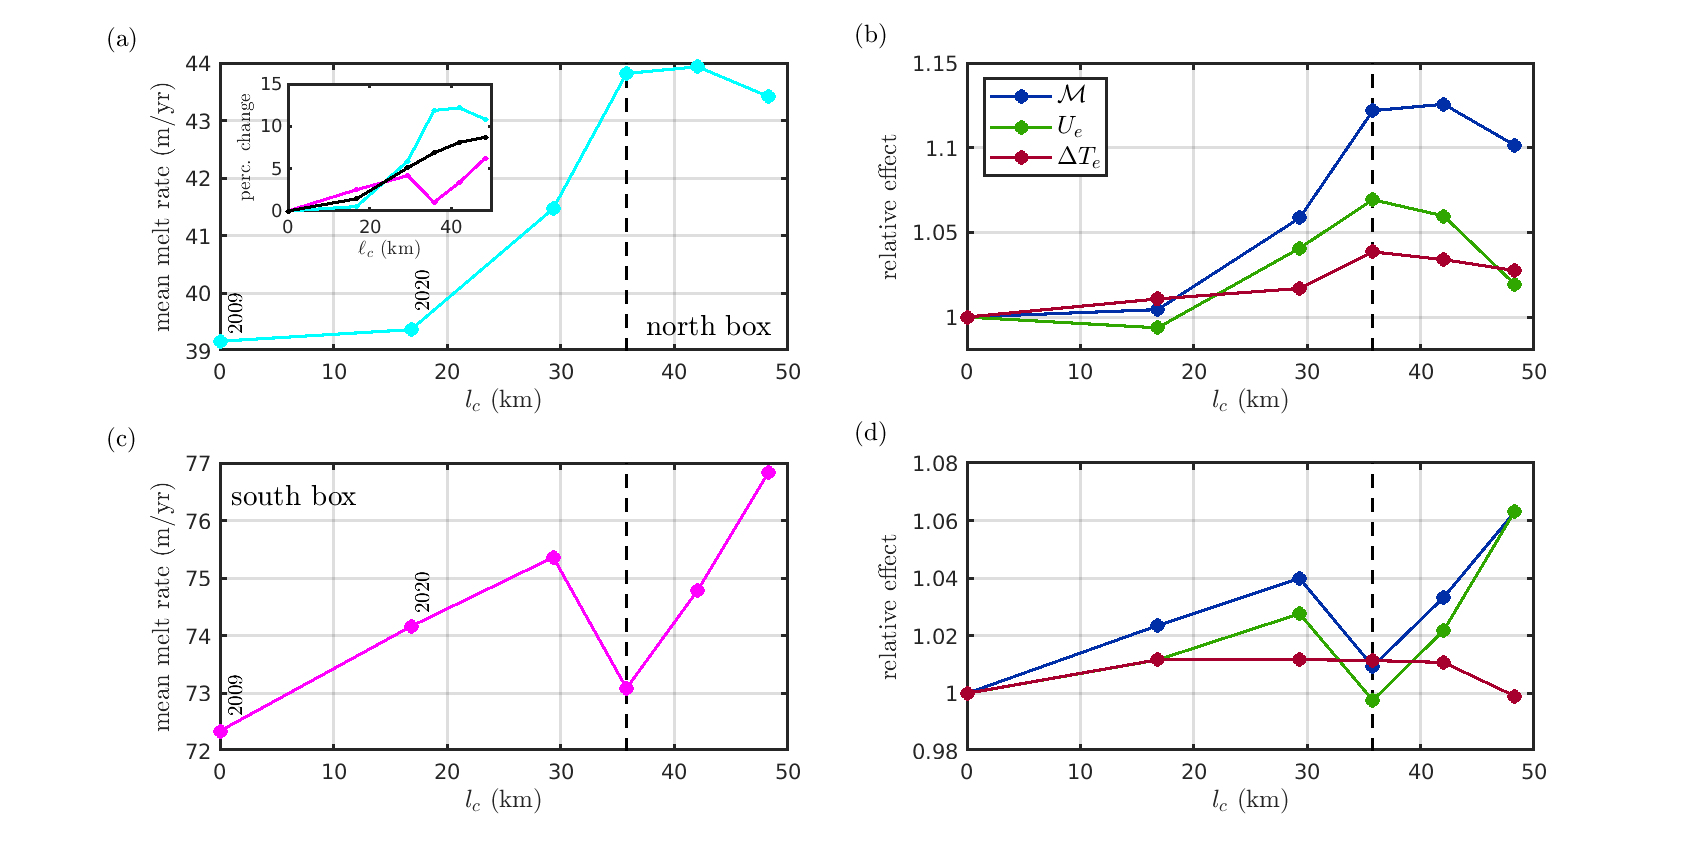
\includegraphics[width = \textwidth]{../make_figures/plots/figure13.png}
    \caption{(a), (c) Average melt rate as a function of calved length $l_c$ in experiments using a PIG geometry. Plots (a) and (c) correspond to the north and south regions of the inner cavity, respectively (cyan and magenta boxes in figure~\ref{fig:figure10}). The calved length $l_c$ is the distance measured along the blue dashed line in figure~\ref{fig:figure10}a, taken relative to the 2009 ice front position (purple curve in figure~\ref{fig:figure10}a). The inset in (a) shows the percentage change in melt rate compared to the uncalved $\ell_c =0$~km (2009) simulation as a function of calved length $\ell_c$ for the north box (cyan curve), south box (magenta curve) and the entire inner cavity region (black curve). (b), (d) Velocity-thermal driving decomposition for the changes in melt rate shown in (a) and (c), respectively. As indicated by the legend in (b), blue, red, and green curves correspond to simulated changes $\mathcal{M}$, velocity effects $U_e$, and thermal driving effects $\Delta T_e$, respectively. In each of the plots, the black dashed line approximately corresponds to the calved length when the ice front sits approximately above the ridge crest.}\label{fig:figure13}
\end{figure}

%these qualitative observations sort of agree with the mean melt rate plots
We show in figure~\ref{fig:figure13}a and c the mean melt rate as a function of calved length for the northern and southern inner cavity regions, respectively. In the northern inner cavity region, the mean melt rate remains approximately constant until the ice front approaches the seabed ridge, where they increase sharply, before remaining approximately constant as the ice front is retreated further. In the southern inner cavity region, the mean melt rate are less variable (in terms of percentage change), but the overall trend is that it increases while the ice front is located downstream of the seabed ridge, before dropping temporarily when the ice front is retreated to the ridge and subsequently increasing again.  More quantitatively, the mean melt rate in the northern inner cavity region reaches a peak that is approximately 12\% larger than present day, which is first realized when the ice front is retreated to the ridge (figure~\ref{fig:figure13}a). Although the mean melt rate in the southern inner cavity region decreases when the ice front is retreated to the ridge (figure~\ref{fig:figure13}c), the combined effect is to increase the melt rate in the entire inner cavity (inset in figure~\ref{fig:figure13}a). Indeed, the melt rate in the entire inner cavity increases approximately linearly after the first calving event (inset in figure~\ref{fig:figure13}a).



%northern box 'hides' behind a narrow gap -- make comparison with the narrow idealized case
Our interpretation of these results is guided by the idealized simulations presented in \S\ref{S:Baseline}--\ref{S:Results:P}. The northern inner cavity region is shielded by a relatively narrow gap between the seabed ridge and the ice draft (inset of figure~\ref{fig:figure10}a), and its melt response to calving behaves in a qualitatively similar way to idealized results with narrower gaps ($W\leq150$~m). A velocity-thermal driving decomposition of these changes in melt rates (figure~\ref{fig:figure13}b) indicates that, as in the corresponding idealized case, both increases in thermal driving and velocity contribute to the increases in melt rate with calving while the ice front is located offshore of the ridge, and that a reduction in the boundary layer velocity is responsible for the decrease in melt rates when the ice front is retreated beyond the ridge. This suggests that the enhancement in melt rates with calving while the ice front is located offshore of the ridge is driven by increased heat reaching the inner cavity and a concomitant increase in buoyancy forcing and thus circulation strength. As in the idealized case, when the calving front reaches the ridge, the trend of increasing melt rate with calving is reversed, although in this case that is observed as a saturation of the melt rates, rather than a strong reduction, as in the idealized case.

%In the idealized case, however, the effect of a reduction in the boundary layer velocity was stronger, and the decrease in melt rate larger, than in this realistic case; we attribute this difference to the splitting of a connected domain into two sub-regions, and the particular complexities of the realistic cavity.

%southern box 'hides' behind a wide gap -- make comparison with the wide idealized case
The southern inner cavity region sits inshore of a relatively wide gap between the seabed ridge and the ice draft (figure~\ref{fig:figure10}). As was the case for idealized simulations with wide gaps ($W\geq200$~m), the mean melt rate is less sensitive to the ice front position than it is with a narrow gap, i.e. for the northern box (inset in figure~\ref{fig:figure13}a). This reduced response suggests that the southern inner cavity is dynamically connected to the outer cavities, regardless of ice front position; barotropic flow, providing significant heat to the inner cavity, is able to cross the ridge to the southern inner cavity in each simulation and thus calving only has limited influence. 


\section{Discussion}\label{S:Discussion}
%loss of area led to increase in speed, but did it also lead to increase in melting which might promote further buttressing loss? Yes at the ice front, but not at GL or shear margins. This suggests negative feedback
The results of the previous section suggest that the recent calving of PIG did not led to increases in melting in either the shear margins or near the grounding line, which are particularly important for buttressing of the grounded ice sheet~\cite{Reese2018NatureClimCh}. Therefore, we do not expect that further buttressing losses associated with increased shelf melting will take place as a result of the recent calving. This lack of response might promote a negative feedback on ice shelf loss, encouraging its regrowth: the recent calving led to an acceleration of the grounded ice~\cite{Joughin2021ScienceAdv}, and thus an increase of the flux of ice into the shelf (assuming that ice thickness at the grounding line remained unchanged); to maintain a constant ice shelf mass balance, melting must therefore increase. The lack of increase in melting after the 2020 calving event might have, therefore, shifted the shelf mass balance towards positive, promoting regrowth of the ice shelf.

However, in all future scenarios considered here (all future ice front positions), further ice front retreat results in an increase in melting. This means that the first chain in the calving-melt feedback loop (calving leads to increased melting, reduced buttressing, acceleration and damage and thus further calving) is never broken, supporting the suggestion that such feedbacks are possible in West Antarctica. However, investigating the detailed response of the ice shelf mass balance to calving event requires the use of a coupled ice-ocean model, and is beyond the scope of this study.

Our results suggest that the mean melt rate in the inner cavity will increase approximately linearly with calving beyond the 2020 front, and in particular, that  the mean inner cavity melt rate will have increased by approximately 10\% when the calving front sits above the ridge. A 10\% increase in melt rates in the inner cavity region corresponds to a increased mass loss of approximately 3~Gt/year, and could represent an important contribution to ice shelf mass inbalance. In addition, this increased mass loss only reflects changes the inner cavity regions, which are small fraction of the total ice shelf area; perhaps more important would be the effect of a 10\% increase in melting in the vicinity of the grounding line, which is particularly important for buttressing the ice sheet, as mentioned. In addition, the spatial pattern of changes in melting indicates that these increases are often focused around the shear margins, which, in addition to being particularly important for buttressing, are the areas most prone to damage and where cracks in ice shelves are often initiated.

The magnitude of changes in melting in response to calving for the southern inner cavity region (for which the offshore ridge-seabed gap is wide) are similar to the corresponding idealized simulations, i.e. reasonably small. For the northern inner cavity region (narrow ridge-seabed gap), however, the magnitude of changes in melt with calving is smaller than the corresponding idealized experiments predict, although the changes are qualitatively similar. We attribute this difference in magnitude to the complexities of the ice draft and seabed in the realistic simulations, and our splitting of the inner cavity into two subsections, which relies on the assumption that they are entirely dynamically disconnected. Although a strong BPV barrier exists between them, some flow is able to cross this barrier, providing a connection between the two regions. This inner cavity decomposition is a convenient tool that permits us to account for some of the effect of the inhomogeneity in ridge-draft gap along its length, but further work is required to fully understand the role of variations in the ridge-draft gap in controlling basal melt rates on PIIS.

In addition, the sensitivity to cavity geometry identified in the idealized simulations means that the observed response may in fact be somewhat different to that predicted here: if, for example, the ridge-draft gap is, in practice, smaller than that used in our realistic simulations (there are reasonable uncertainties in the ice draft and bathymetry beneath the shelf), the melt response to calving might be significantly larger. Furthermore, the ice draft is not static but varies dynamically; advection of thicker sections of the ice shelf to the ridge crest would be expected to narrow the ridge-draft gap and thus increase the sensitivity of melt rates to calving, and vice versa for the advection of thinner sections of ice. Our idealized simulations also suggest that the melt-gap geometry feedback identified by~\cite{DeRydt2014JGeophysResOceans}, in which increases in the ridge-draft gap lead to an increase in melt rate and thus further ridge-draft gap widening, holds for any ice front position offshore of the ridge.

Variability in the depth of the pycnocline dominates ocean variability in the Amundsen Sea on decadal timescales. Our idealized simulations point to a reduction in the sensitivity to pycnocline depth with calving once the ice front is reasonably close to the ridge provided that the gap is relatively thin ($l_c > 20$~km on the inset of figure~\ref{fig:figure8}a, which is appropriate for $W=100$~m). However, for thicker gaps ($W > 150$~m), the sensitivity to pycnocline depth is largely independent of the ice front position (figure~\ref{fig:figure8}a, b). This conclusion is also borne out in our realistic experiments: supplementary experiments (not shown) using the realistic geometry, with the ocean restored to 2012 conditions in PIB far from the ice shelf, reveal that the ratio between the mean melt rate in the norther inner cavity region (narrow gap) for 2009 and 2012 boundary conditions is 1.52 for the largest ice shelf we consider, and 1.43 for the smallest. However, for the southern inner cavity region (wide gap), this ratio shows little change between the largest (1.29) and smallest (1.31) ice shelves we consider. The combination of a reduction in sensitivity in the northern box and an invariance in the southern box as calving proceeds suggests that PIIS melting may experience a reduction in the sensitivity to ocean conditions in the Amundsen Sea in the future, assuming that the ice front continues to retreat. This motivates further study into future changes of the sensitivity of Amundsen Sea sector ice shelves to far field oceanic conditions.

The results presented in this paper have implications for melt rate parametrizations. At present, no melt rate parametrization is able to account for the position of the ice front, seabed topography, or indeed any BPV barrier, when computing the melt rate~\cite{AsayDavis2017CurrClimChRep, Reese2018Cryo, Bradley2022}. Although the example of PIG is somewhat extreme in this BPV barrier sense, we have demonstrated that the combination of seabed ridge and ice front position, which ultimately act as BPV barriers, can be an important control on the melt rate applied to an ice shelf. Ultimately, our results suggest that current melt rate parametrizations must be improved to account for the seabed ridge if they are to be trusted in future projections of PIIS.

It is important to note that MITgcm has a plethora of parameter choices and numerical settings, which might have an impact on the results of the simulations. These include choices of grid resolution, which are $400$~m in the horizontal (to ensure mesoscale eddies are well resolved) and $10$~m in the vertical. Simulations at higher vertical resolution ($5$~m) did not change the results significantly, although results were somewhat different for lower resolution ($20$~m); this is perhaps unsurprising given that exchange over the ridge crest, which we have shown to be important in controlling the inner cavity melt rate, is expected to be sensitive to vertical resolution. Agreement with the higher resolution simulations gives us confidence that the simulations presented here are appropriately resolving exchange processes over the ridge crest.

Finally, it is important to note that forcing in our simulations comes exclusively from buoyancy fluxes associated with ice shelf melting and restoring at the boundaries. In particular, the simulations include neither surface heat and freshwater fluxes nor sea ice, which would be expected to alter the horizontal density gradients and thus circulation in the open ocean. In addition, they do not include wind stresses, which provide a leading order control on heat content and circulation in Pine Island Bay~\cite{Dutrieux2014Science}.

\section{Summary}\label{S:Summary}
%general overview of the question and answer
The central aim of this study is to understand how, and why, melt rates on Pine Island Ice Shelf might respond to calving events that have already taken place recently, and those that might occur in the future. To address this question, we have performed numerical simulations in both an idealized domain, and one that is representative of PIIS.

The idealized experiments allowed us to isolate parametric dependencies in the melt response to calving, and elucidate the mechanisms responsible for it. We identified a sensitive dependency on the cavity geometry via the parameter $W$ that describes the gap between the seabed ridge and the ice draft: configurations with a narrow gap ($W \lesssim 150$~m) have a large response to calving, whereas those with wide gaps ($W>150$~m) do not. We identified two key regimes for configurations whose cavities has a narrow gaps: in the first, the ice front is located offshore of the ridge, and the inner cavity melt rate increases with calving, and the change in melting for a given calved length increases as the ice front approaches the ridge. In the second regime, the ice front is located at or inshore of the ridge, and melt rates are significantly reduced compared to when the ice front is just offshore of the ridge if the pycnocline is relatively high, or enhanced further if the pycnocline is relatively deep. In contrast, for configurations with wide gaps, the melt rate is largely independent of the location of the ice front. Using a barotropic framework, we identified the roles of changes in circulation and thermal driving in the melt response to calving, and  described how these roles are modulated by barotropic flow across the ridge, meltwater mixing, and barotropic potential vorticity barriers in the domain. Although these idealized results are intended to inform our understanding of melt rate changes beneath Pine Island Glacier, they can also be considered to be an archetype for situations in which the seabed geometry restricts the access of warm water to the grounding line of an ice sheet. This situation might be realized, for example, in ice sheet retreat over an over-deepened bed. In addition, the results for wide gaps suggest that melt rates are insensitive to ice front position in ice shelf cavities with no seabed ridge.

The idealized experiments informed experiments performed using a cavity geometry that closely resembles PIIS, designed to assess how melt rates on PIIS might respond to calving in practice. This geometry has two inner cavity regions, which are approximately dynamically disconnected due to a thick ice keel across the center of the glacier. One of the inner cavity sections sits inshore of a narrow section of the ridge-draft gap; in this region the melt rate increases with calving while the ice front is located offshore of the ridge, before saturating with further calving beyond the ridge. In contrast, the other cavity section sits inshore of a wide section of the ridge-draft gap; there, the melt rate is largely independent of calving. Both of these observations are qualitatively consistent with the idealized simulations. %By making an analogy with the idealized results, we suggest that the same competing mechanisms of heat access to the inner cavity and topographic confinement of the circulation are responsible.

Our results demonstrate that the impact of calving on melt rates may represent an important, but as yet unexplored, contribution to the ice-ocean sensitivity of the West Antarctic Ice Sheet. They provide evidence that melt rates have not changed in response to recent calving events, but will increase linearly with future calving events. This increased mass loss, which is expected to take place in dynamically important regions of the ice shelf, might lead to a significant ice shelf mass imbalance. In addition, the constant increase in melt rate with retreat supports the possibility of a feedback loop in which calving leads to increased melting, reduced buttressing, acceleration and damage and thus further calving.

\acknowledgments
A. T. B. and D. T. B. are supported by the NERC Grant NE/S010475/1. J. D. R. is supported by the TiPACCs project, which receives funding from the European Union's Horizon 2020 research and innovation programme under grant agreement no. 820575. NSF (through grant OPP-1643285) and the NASA MAP program provided support to P.D..

The simulations were performed using MITgcm at checkpoint c67u, which is publicly accessible at \url{http://mitgcm.org/public/source_code.html}. Files and code used to drive MITgcm and produce the figures in this paper are available at \url{https://github.com/alextbradley/PIG-melt-reponse-to-calving}.

The numerical simulations were carried out on ARCHER2, the U.K. national HPC facility (\url{http://archer2.ac.uk/}).

\bibliography{mybib}


\end{document}
